\documentclass[11pt,a4paper]{article}
\usepackage[T1]{fontenc}
\usepackage{lmodern}
\usepackage[margin=2.5cm]{geometry}
\usepackage{amsmath,amssymb,amsthm}
\usepackage{booktabs}
\usepackage{array}
\usepackage{enumitem}
\usepackage{xcolor}
\usepackage{graphicx}
\graphicspath{{figures/}}
\PassOptionsToPackage{hyphens}{url}
\usepackage[colorlinks=true,linkcolor=blue!50!black,urlcolor=blue!50!black]{hyperref}

\renewcommand{\Re}{\operatorname{Re}}
\renewcommand{\Im}{\operatorname{Im}}
\newcommand{\dext}{\delta_{\rm ext}}
\newcommand{\Lop}{\mathcal{L}_\ell}
\newcommand{\PhiS}{\Phi^{\rm S}}
\newcommand{\PhiR}{\Phi^{\rm R}}
\newcommand{\phiS}{\phi^{\rm S}}
\newcommand{\phiR}{\phi^{\rm R}}
\newcommand{\x}{\mathbf{x}}
\newcommand{\nb}[1]{\nolinkurl{#1}}
\newcommand{\code}[1]{\texttt{#1}}

\newtheorem{proposition}{Proposition}
\newtheorem{lemma}{Lemma}

\title{Which singular field?\\[4pt]
\large Keeping the S/R split consistent between the first-order contour solve\\ and the second-order source}
\author{Draft prepared with Claude Code for Andrew Spiers (UCD)}
\date{6 October 2026}

\begin{document}
\maketitle

\begin{abstract}
The plan for the second-order problem splits the first-order field as $\Phi_1=\PhiS+\PhiR$ and the second-order source into singular--singular (SS), singular--regular (SR) and regular--regular (RR) pieces.
SS and SR are built from closed-form 3D expressions for $\PhiS$.
SR and RR use the mode-decomposed $\PhiR$, which the first-order solve produces on the contour.
This only works if every piece uses \emph{the same} singular field.
This note explains how the singular mode in the current first-order notebook can differ from the $\ell$-mode of the 3D singular field by a homogeneous solution of the radial equation.
An explicit example shows that the difference need not be small: it can be the entire Coulomb field outside the sphere $r=r_0$.
The note also identifies a second, independent freedom in the imaginary part (the ``shadow'') of the singular mode, and gives conditions and a construction that remove both.
The first requirement is the same consistency condition that traditional real-axis puncture schemes satisfy by construction.
The second has no real-axis counterpart and is specific to the contour.
A Mathematica implementation of the $1/\rho^2$ and $1/\rho^4$ cases confirms the prescription: exterior second-order errors are at the level of $10^{-16}$. For $1/\rho^4$, the contour picks the Hadamard finite part with no point-supported terms.
It also shows that the shadow from a truncated puncture is of the same order as the puncture's own truncation error.
With a truncated 3D puncture, that shadow grows with the number of coupled modes.
Two remedies restore convergence: shrinking the worldtube as modes are added, or a hybrid split that forms the regular part of SR on the real line and continues it with a Cauchy integral.
A test with a distributional SR, whose modes contain $\delta$-function terms, shows that the hybrid split still works where a purely real-line treatment fails.
Finally, the contour reproduces the mode-level Hadamard regularisation of Musaeus, Pound and Upton to $10^{-34}$, including Teukolsky-type $1/\Delta r^4$ sources.
Applied to the canonical source, it also captures their worldline term $T_Q$ automatically.
\end{abstract}

{\small\tableofcontents}
\clearpage

\section{Context and scope}

The notebook \nb{Singular-and-regular-split-works-real-outside-worldtube.nb} shows that the regular part of the first-order field can be recovered on a complex contour inside a worldtube around the particle.
It uses an effective source $\dext-\Lop[\phiS_{\rm local}]$.
The plan for second order is to write the source, a symmetric bilinear operator $Q$ acting on $\Phi_1$, as
\begin{equation}
Q[\Phi_1,\Phi_1]=\underbrace{Q[\PhiS,\PhiS]}_{\rm SS}+\underbrace{2Q[\PhiS,\PhiR]}_{\rm SR}+\underbrace{Q[\PhiR,\PhiR]}_{\rm RR}.
\label{eq:split}
\end{equation}
The pieces are computed as follows:
\begin{itemize}[nosep]
\item SS from 3D formulas, with no mode decomposition of the first-order field.
\item SR from the 3D singular field combined with the mode-decomposed $\PhiR$.
\item RR from the mode-decomposed $\PhiR$.
\end{itemize}

\paragraph{Decisions (6 October 2026).}
\begin{enumerate}[nosep]
\item Work first with $Q[A,B]=AB$, so that SS $=q^2/\rho^2$.
  Keep every step general enough for $Q[A,B]=\nabla A\cdot\nabla B$, where SS $=q^2/\rho^4$; this is the original problem in \nb{Modes-of-Source-and-solution-1or4.nb}.
\item Solve RR on the real line.
\item Compute $\PhiR$ on the real line as well as on the contour.
  RR needs it on the real segment inside the worldtube; SR needs its continuation onto the contour.
\item The primary output is $\Phi_2$ \emph{outside} the worldtube.
  This is the analogue of the fluxes at the horizon and at null infinity, which suffice for first-post-adiabatic models.
  The value at the particle is a secondary goal.
\end{enumerate}

This note addresses the first open question.
The singular field used in the first-order contour solve must be the mode decomposition of the same 3D singular field that is used in SS and SR.
More precisely, it must be the mode decomposition of the same 3D \emph{puncture}.
Section~\ref{sec:traditional} compares this with traditional puncture schemes.

\section{Setup and conventions}

\subsection{Toy model}
The toy model is flat space with a particle of charge $q$ at $\x_0=r_0\hat{\mathbf z}$, and $\rho=|\x-\x_0|$.
The first-order field satisfies
\begin{equation}
\nabla^2\Phi_1=-4\pi q\,\delta^3(\x-\x_0),
\end{equation}
with boundary conditions on the computational domain (the notebooks use $r\in[1,10]$) that inject a regular field.
I take $\PhiS=q/\rho$, the toy analogue of the Detweiler--Whiting singular field.
Then $\PhiR:=\Phi_1-\PhiS$ is harmonic near $\x_0$.
At second order, $\nabla^2\Phi_2=Q[\Phi_1,\Phi_1]$.

\subsection{Modes}
With axisymmetry, $\Phi(\x)=\sum_\ell\phi_\ell(r)\,Y_\ell(\theta)$, where $Y_\ell\equiv Y_{\ell0}$, and $[\nabla^2\Phi]_\ell=\Lop\phi_\ell$ with
\begin{equation}
\Lop\psi=\psi''+\frac{2}{r}\psi'-\frac{\ell(\ell+1)}{r^2}\psi .
\end{equation}
The first-order mode equation is $\Lop\phi_{1,\ell}=\kappa_\ell\,\delta(r-r_0)$, with
\begin{equation}
\kappa_\ell=-\frac{4\pi q}{r_0^2}Y_\ell(0)=-\frac{q}{r_0^2}\sqrt{4\pi(2\ell+1)}.
\end{equation}
The split notebook uses unit strength, $\kappa_\ell=1$, and so do I below; $\kappa_\ell$ is restored when converting back to 3D.
(The notebooks use different normalisations: \nb{Greens-function-Poisson-equation-3.nb} uses a $-4\pi\delta^3$ source.
The implementation should fix one.)

The unit-strength $\ell$-mode of the Coulomb field is
\begin{equation}
G_\ell(r)=-\frac{r_0^2}{2\ell+1}\,\frac{r_<^\ell}{r_>^{\ell+1}},\qquad r_<=\min(r,r_0),\quad r_>=\max(r,r_0).
\label{eq:G}
\end{equation}
It is the unique solution of $\Lop G_\ell=\delta(r-r_0)$ that is regular at $r=0$ and decays as $r\to\infty$.
Moreover, $\kappa_\ell G_\ell=q\sqrt{4\pi/(2\ell+1)}\,r_<^\ell/r_>^{\ell+1}$ is exactly the $\ell$-mode of $q/\rho$.

\subsection{Extended delta, contour and shadows}
Define
\begin{equation}
H(z)=1+\frac{i}{\pi}\log(z-r_0),\qquad \dext(z)=H'(z)=\frac{i}{\pi(z-r_0)},
\end{equation}
using the principal logarithm.
The contour $z=y(a)$ lies in the closed upper half-plane and coincides with the real axis outside the worldtube $[a_L,a_R]$.
Real-axis values are boundary values from above.
This is also Mathematica's convention, $\code{Log}[-x]=\ln x+i\pi$.
By the Sokhotski--Plemelj formula,
\begin{equation}
H(r+i0)=\Theta(r-r_0)+\frac{i}{\pi}\ln|r-r_0|,\qquad
\dext(r+i0)=\delta(r-r_0)+\frac{i}{\pi}\,\mathrm{P}\frac{1}{r-r_0}.
\label{eq:SP}
\end{equation}
The real parts are the physical objects; the imaginary parts are the shadows of \nb{Andrew_s_idea.pdf}.

\begin{lemma}[Linear solves on the contour]\label{lem:linear}
Suppose that:
\begin{itemize}[nosep]
\item $\tilde s$ is analytic in the part of the worldtube above the real axis;
\item $\Re\tilde s(r+i0)=s(r)$ on the real segment, as distributions;
\item $\tilde\psi$ solves $\Lop\tilde\psi=\tilde s$ along the contour, starting from real data at $a_L$.
\end{itemize}
Then $u(r):=\Re\tilde\psi(r+i0)$ solves $\Lop u=s$ on $[a_L,a_R]$ with the same data.
In particular, $\Re\tilde\psi(a_R)$ and $\Re\tilde\psi'(a_R)$ are the values one would get by solving the physical problem on the real line.
\end{lemma}
\noindent\emph{Proof sketch.}
The coefficients of $\Lop$ are analytic away from $z=0$.
So the solution continued along the contour equals the boundary value from above of the solution in the region between the contour and the real axis.
The coefficients are also real, so $\Lop$ commutes with taking the real part. \qed

\medskip
Everything linear works because of Lemma~\ref{lem:linear}.
Products do not: for $\tilde\psi_1=u_1+iv_1$ and $\tilde\psi_2=u_2+iv_2$,
\begin{equation}
\Re(\tilde\psi_1\tilde\psi_2)=u_1u_2-v_1v_2,
\end{equation}
as in \S2 of \nb{Andrew_s_idea.pdf}.
The split \eqref{eq:split} avoids this provided every product is formed in one of two ways:
\begin{itemize}[nosep]
\item on the real configuration, before continuation (SS, built analytically from 3D);
\item with at most one factor carrying a shadow (SR).
\end{itemize}
The second requirement is the job of $\PhiR$.
Because $\PhiR$ is smooth at $\x_0$, its modes on the contour should be analytic continuations of real functions, with no shadow.
Sections~\ref{sec:two}--\ref{sec:imag} show that this is not automatic.

\section{Two candidate singular modes}\label{sec:two}

\paragraph{(A) The 1D singular mode used in the notebook.}
The notebook defines
\begin{equation}
\psi_p:=\code{DSolveValue}[\Lop\psi=\dext,\ \psi,\ r]\ \text{with}\ \code{C[\_]}\to0
\end{equation}
(\code{singularModeExact}).
The puncture is its expansion about $r_0$ through order $n$ (\code{phiSLocal}).
This mode is chosen by a \emph{local} property: it carries the $\log(z-r_0)$ singular structure forced by $\dext$.

\paragraph{(B) The $\ell$-mode of the 3D singular field.}
On the real line this is $\phiS_\ell=\kappa_\ell G_\ell$, or $G_\ell$ at unit strength.
SS and SR use it implicitly when they are built from $q/\rho$.

\medskip
The question is whether $\Re\psi_p(r+i0)=G_\ell(r)$.
In general it is not.

\section{How they can differ by a homogeneous solution}\label{sec:homog}

\begin{proposition}\label{prop:homog}
Let $\psi$ be any solution of $\Lop\psi=\dext$ that is analytic in the upper half of a neighbourhood of an interval $[r_{\min},r_{\max}]\ni r_0$, with $r_{\min}>0$.
Then
\begin{equation}
D(r):=\Re\psi(r+i0)-G_\ell(r)=\alpha\,r^\ell+\beta\,r^{-\ell-1},\qquad \alpha,\beta\in\mathbb R .
\end{equation}
\end{proposition}
\begin{proof}
$\Lop$ has real, analytic coefficients on $(r_{\min},r_{\max})$.
Taking boundary values and real parts therefore commutes with $\Lop$, so by \eqref{eq:SP}
\[
\Lop\,\Re\psi(r+i0)=\Re\dext(r+i0)=\delta(r-r_0).
\]
$G_\ell$ satisfies the same equation, so $\Lop D=0$ in the sense of distributions.
Since $\Lop$ has smooth coefficients there, $D$ is a classical solution, that is, a combination of $r^\ell$ and $r^{-\ell-1}$.
\end{proof}

\paragraph{Interpretation.}
The source fixes only the \emph{singular structure} at $r_0$:
\begin{itemize}[nosep]
\item On the real line, $\psi$ is continuous with $[\psi']=1$.
\item In the complex plane, $\psi$ contains a term $\frac{i}{\pi}h_\ell(z)\log(z-r_0)$, where $h_\ell$ is homogeneous with $h_\ell(r_0)=0$ and $h_\ell'(r_0)=1$.
\end{itemize}
The homogeneous solutions $r^\ell$ and $r^{-\ell-1}$ are smooth at $r_0>0$, so no condition imposed at $r_0$ can see them.
A singular mode therefore needs two further conditions:
\begin{itemize}[nosep]
\item $G_\ell$ gets them from 3D: regularity at the origin and decay at infinity, so that the mode sum reconstructs $q/\rho$.
\item $\psi_p$ gets them from whichever antiderivatives \code{DSolve} happened to choose before \code{C[\_]} was set to $0$.
\end{itemize}
The notebook comment that the singular field ``is a LOCAL property'' is true of its singular structure.
It is not true of the smooth part that comes with it.

\subsection{An explicit example}
Use variation of parameters with $y_1=r^\ell$, $y_2=r^{-\ell-1}$ and Wronskian $W=-(2\ell+1)/r^2$:
\begin{equation}
\psi_p(z)=\frac{1}{2\ell+1}\left[z^\ell\!\int^z\! s^{1-\ell}\dext(s)\,ds-z^{-\ell-1}\!\int^z\! s^{\ell+2}\dext(s)\,ds\right].
\end{equation}
Evaluate the antiderivatives by partial fractions with real coefficients and no extra constants.
The only non-real ingredient is $\log(z-r_0)$, with coefficients $r_0^{1-\ell}$ and $r_0^{\ell+2}$ respectively.
Hence
\begin{equation}
\psi_p(z)=\frac{i}{\pi}\Big[h_\ell(z)\log(z-r_0)+p_\ell(z)\Big],\qquad
h_\ell(z)=\frac{r_0^{1-\ell}z^\ell-r_0^{\ell+2}z^{-\ell-1}}{2\ell+1},
\end{equation}
where $p_\ell$ (polynomials, powers of $z$ and $\log z$) is real for $z>0$.
For example, $\psi_p=\frac{i}{\pi}\big[(r_0-r_0^2/z)\log(z-r_0)+z/2-r_0\big]$ for $\ell=0$.

The boundary values on the real line are:
\begin{itemize}[nosep]
\item for $r>r_0$, everything is $i\times$real, so $\Re\psi_p=0$;
\item for $r<r_0$, $\log(r-r_0+i0)=\ln|r-r_0|+i\pi$, so $\Re\psi_p=-h_\ell$.
\end{itemize}
Therefore
\begin{equation}
\Re\psi_p(r+i0)=-h_\ell(r)\,\Theta(r_0-r).
\end{equation}
This is a \emph{one-sided} Green's function, which vanishes identically for $r>r_0$.
Comparing with \eqref{eq:G},
\begin{equation}
D_\ell(r)=\Re\psi_p(r+i0)-G_\ell(r)=\frac{r_0^{\ell+2}}{2\ell+1}\,r^{-\ell-1}\qquad\text{on both sides of }r_0,
\label{eq:Dl}
\end{equation}
as Proposition~\ref{prop:homog} requires.
For the notebook's $\ell=2$ this gives $D_2=r_0^4/(5r^3)$.

\paragraph{The difference in 3D.}
Using $\sqrt{4\pi(2\ell+1)}\,Y_\ell(\theta)/(2\ell+1)=P_\ell(\cos\theta)$ and the Legendre generating function,
\begin{equation}
\Delta(\x):=\sum_\ell\kappa_\ell D_\ell(r)Y_\ell(\theta)
=-\frac{q}{r_0}\sum_\ell\Big(\frac{r_0}{r}\Big)^{\ell+1}P_\ell(\cos\theta)
=\begin{cases}-q/\rho, & r>r_0,\\ \text{divergent}, & r<r_0.\end{cases}
\end{equation}
So $\psi_p$ is not ``the Coulomb mode plus a small correction''.
In 3D its real part is the Coulomb field minus the \emph{entire} Coulomb field outside the sphere $r=r_0$.

The antiderivative could instead be written with $\log(r_0-z)$, which is also analytic in the upper half-plane.
That gives the mirror image: $\Re\psi_p$ vanishes for $r<r_0$, $D_\ell=r_0^{1-\ell}r^\ell/(2\ell+1)$, and the sum is $-q/\rho$ for $r<r_0$.

\paragraph{What \code{DSolve} actually returns.}
The example above assumes real-coefficient antiderivatives written with $\log(z-r_0)$.
The Mathematica implementation (Section~\ref{sec:numerics}) evaluated the notebook's \code{singularModeExact} directly.
\code{DSolve} writes its antiderivatives with $\log(r_0-z)$, together with $\log(z-r_0)$ for $\ell=0,1$ or $\log z$ for $\ell\ge2$.
Proposition~\ref{prop:homog} holds exactly: $\alpha$ and $\beta$ were fitted at two points and verified at 17 others, on both sides of $r_0$.
\begin{center}
\small
\renewcommand{\arraystretch}{1.2}
\begin{tabular}{@{}cccl@{}}
\toprule
$\ell$ & $\alpha$ & $\beta$ & $\Re\psi_p(r+i0)$\\
\midrule
$0$ & $r_0$ & $r_0^2$ & $r_0^2/r$ inside, $r_0$ outside: an anti-physical Green's function\\
$1$ & $0$ & $0$ & $G_1$, the physical Coulomb mode\\
$2$--$12$ & $r_0^{1-\ell}/(2\ell+1)$ & $0$ & the mirror case: zero for $r<r_0$\\
\bottomrule
\end{tabular}
\end{center}
In 3D, for $r<r_0$, $\sum_\ell\kappa_\ell D_\ell Y_\ell=-q/\rho+q\,r\cos\theta/r_0^2-q/r$; for $r>r_0$ the sum diverges.
The conclusions of Section~\ref{sec:matters} therefore apply to the notebook as it stands.

\section{Why it matters}\label{sec:matters}

\subsection{At first order it is only a relabelling}
With choice (A), the ``regular'' field is $\PhiR_A:=\Phi_1-\PhiS_A=\PhiR-\Delta$.
Each mode $\phiR_{A,\ell}=\phiR_\ell-\kappa_\ell D_\ell$ is still smooth at $r_0$ and still solves the homogeneous mode equation.
The notebook is self-consistent because it \emph{defines} the full field as (regular)\,$+\,\psi_p$.
A purely 1D test cannot detect the difference.

In 3D, however, the difference is not harmless.
In the one-sided example, $\PhiR_A=\PhiR+q/\rho=\Phi_1$ for $r>r_0$.
The ``regular'' field then contains the whole Coulomb field outside the sphere and is singular at $\x_0$ when approached from outside.
Its mode sum converges no faster than that of $\Phi_1$, and for $r<r_0$ it does not converge at all.
\emph{Smoothness of every mode at $r_0$ does not imply regularity in 3D.}
Regularity in 3D comes only from the 3D definition of $\PhiS$.

\subsection{At second order it changes the answer}
Suppose SS and SR are built from $\PhiS=q/\rho$, but SR and RR use $\PhiR_A$.
By bilinearity,
\begin{equation}
Q[\PhiS,\PhiS]+2Q[\PhiS,\PhiR_A]+Q[\PhiR_A,\PhiR_A]
=Q[\Phi_1-\Delta,\Phi_1-\Delta]
=Q[\Phi_1,\Phi_1]-2Q[\Phi_1,\Delta]+Q[\Delta,\Delta].
\end{equation}
This is the second-order source of the \emph{wrong} first-order field, and it fails in two ways:
\begin{itemize}[nosep]
\item The error contains $-2Q[\PhiS,\Delta]$, which is $-2q\Delta/\rho$ in the $1/\rho^2$ case.
  This is singular at $\x_0$ unless $\Delta$ vanishes there, so it even changes the singular structure that SS is meant to capture.
\item The RR mode coupling loses the fast convergence the plan relies on, because $\PhiR_A$ is not smooth in 3D.
\end{itemize}
Using $\PhiS_A$ \emph{consistently} everywhere would make the split algebraically exact again.
But SS and SR need $\PhiS_A$ as a 3D field, and it has none: in the example its mode sum diverges for $r<r_0$.
So the real requirement is not ``use $q/\rho$''.
It is ``use one 3D puncture field, which can be evaluated in closed form, in every piece''.
Section~\ref{sec:traditional} makes this precise.

\section{A second freedom: the imaginary part of the singular mode}\label{sec:imag}

\subsection{What SR needs}
Fixing $\Re\phiS_\ell$ on the real line leaves its continuation off the axis undetermined.
On the contour, the SR source contains products $\tilde F(z)\,\tilde\phi^{\rm R}_{\ell'}(z)$, where $\tilde F$ is a continued coupling function (Section~\ref{sec:second}).
On the real axis,
\begin{equation}
\Re(\tilde F\tilde\phi^{\rm R})=\Re\tilde F\,\Re\tilde\phi^{\rm R}-\Im\tilde F\,\Im\tilde\phi^{\rm R}.
\end{equation}
Lemma~\ref{lem:linear} gives the physical SR result only if $\Im\tilde\phi^{\rm R}(r+i0)=0$, that is, only if $\tilde\phi^{\rm R}$ is the analytic continuation of the real $\phiR$.
Since $\tilde\phi^{\rm R}$ solves $\Lop\tilde\phi^{\rm R}=\dext-\Lop\phiS$ with real data at $a_L$, this holds exactly when
\begin{equation}
S_{\rm eff}:=\dext-\Lop\phiS_\ell\ \text{ is real on the real axis}
\label{eq:C2}
\end{equation}
(with $S_{\rm eff}=0$ for the exact singular mode).

\subsection{Why replacing $\Theta$ by $H$ does not do this automatically}
$\dext$ is not localised at $r_0$ in the way $\delta$ is.
For $f$ analytic and real on the real axis,
\begin{equation}
f(z)\dext(z)=f(r_0)\dext(z)+\frac{i}{\pi}\,\frac{f(z)-f(r_0)}{z-r_0},\qquad (z-r_0)^2\dext'(z)=-\frac{i}{\pi},
\end{equation}
whereas $f(r)\delta(r-r_0)=f(r_0)\delta(r-r_0)$ and $(r-r_0)^2\delta'(r-r_0)=0$.
The remainders are smooth and imaginary on the real axis.
So replacing $\Theta\to H$ in a formula that is exact on the real line produces such remainders.
An example of such a formula is the Coulomb mode written as $G_\ell=G_\ell^{\rm in}+(G_\ell^{\rm out}-G_\ell^{\rm in})\Theta(r-r_0)$.

\paragraph{Example, $\ell=0$.}
On the real line, $G_0=-r_0+(r_0-r_0^2/r)\,\Theta(r-r_0)$.
Define $\tilde G_0(z):=-r_0+(r_0-r_0^2/z)H(z)$.
It has the right real part, $\Re\tilde G_0(r+i0)=G_0$, but
\begin{equation}
\mathcal L_0\tilde G_0=\dext(z)-\frac{i}{\pi}\frac{1}{z}.
\end{equation}
Used as a puncture, it leaves $S_{\rm eff}=\frac{i}{\pi}\frac1z$, which is imaginary on the real axis.
The ``regular'' field then acquires $\Im\tilde\phi^{\rm R}=r/(2\pi)+(\text{homogeneous})$.
This shadow is $O(1)$, not small.
The fix is to add a smooth imaginary piece:
\begin{equation}
\phiS_0(z)=\tilde G_0(z)+\frac{i}{2\pi}z,\qquad \mathcal L_0\phiS_0=\dext,\qquad \Re\phiS_0(r+i0)=G_0 .
\end{equation}

\subsection{Imaginary homogeneous solutions are harmless}
Adding $i(\gamma r^\ell+\gamma' r^{-\ell-1})$ with $\gamma,\gamma'$ real to $\phiS_\ell$ changes neither its real part nor \eqref{eq:C2}.
The full field inherits the change in shadow through the matching at $a_L$, and $\tilde\phi^{\rm R}$ is unchanged.

\section{Relation to traditional puncture schemes}\label{sec:traditional}

Write $\Phi^{\rm P}$ for the 3D puncture and $\Phi^{\rm res}:=\Phi_1-\Phi^{\rm P}$ for the residual field.
In the toy model the natural choice is $\Phi^{\rm P}=\PhiS=q/\rho$, for which $\Phi^{\rm res}=\PhiR$.

\subsection{How a real-axis scheme builds its puncture modes}
Effective-source and puncture schemes~\cite{BarackGolbourn2007,VegaDetweiler2008} start from a 4D (here 3D) puncture.
This is a local expansion of the Detweiler--Whiting singular field to some order, usually multiplied by a window function that equals one near the particle, or cut off at a worldtube.
The modes of the puncture are obtained by \emph{projecting that field} onto the harmonics: analytically for $\ell$-mode punctures, by integration for $m$-mode schemes.
A puncture mode is never defined by solving the 1D mode equation with a delta source.
The consistency requirement of Section~\ref{sec:matters} therefore holds by construction.

The 1D route taken in the current notebook is what let the homogeneous ambiguity in.
The extended equation has a convenient closed-form particular solution, and setting \code{C[\_]}\,$\to0$ silently chooses its smooth part.

\subsection{The allowed freedom is the same}
In both settings, the puncture modes may be the modes of \emph{any} 3D field $\Phi^{\rm P}$ whose difference from $\PhiS$ is smooth at $\x_0$, to the order the scheme needs.
Window functions use exactly this freedom.
The residual field is then as regular as $\Phi^{\rm P}-\PhiS$.

A mode-by-mode shift is acceptable only if it is the set of modes of such a 3D field.
A shift by homogeneous solutions, $\sum_\ell\Delta_\ell Y_\ell$, is harmonic wherever the sum converges.
If it converges in a neighbourhood of $\x_0$, it is a legitimate smooth change of puncture.
The one-sided example of Section~\ref{sec:homog} is not: it equals $-q/\rho$ for $r>r_0$ and diverges for $r<r_0$.

\subsection{Where the problem shows up}
\begin{itemize}[nosep]
\item \emph{First order, exterior values.}
  A worldtube scheme solves for the full field outside the worldtube and for the residual field inside, with a jump equal to the puncture at the boundary.
  The exterior field, and hence the fluxes, does not depend on the puncture, as long as the same puncture is used on both sides of the jump.
  This is why the notebook cannot see $\Delta$.
  A traditional first-order flux calculation would not see it either.
\item \emph{First order, at the particle.}
  The self-force needs $\nabla\PhiR(\x_0)$, so the puncture must agree with $\PhiS$ through $O(|\x-\x_0|)$; that is, $\Phi^{\rm P}-\PhiS=O(|\x-\x_0|^2)$.
  A smooth $\Delta$ with $\nabla\Delta(\x_0)\neq0$ would change the self-force.
\item \emph{Second order.}
  The split
  \begin{equation}
  Q[\Phi_1,\Phi_1]=Q[\Phi^{\rm P},\Phi^{\rm P}]+2Q[\Phi^{\rm P},\Phi^{\rm res}]+Q[\Phi^{\rm res},\Phi^{\rm res}]
  \label{eq:splitP}
  \end{equation}
  is an algebraic identity for any $\Phi^{\rm P}$, provided the same $\Phi^{\rm P}$ appears in all three pieces and in the definition of $\Phi^{\rm res}$.
  Traditional second-order puncture schemes rely on the same condition.
  In those schemes the pieces containing the puncture are computed from 4D expressions, and only the residual pieces by mode coupling.
  This is the strategy used against the infinite mode-coupling problem~\cite{MillerWardellPound2016}.
  Condition (C3) below is exactly this condition.
\end{itemize}

\subsection{What is new on the contour}
\begin{itemize}[nosep]
\item \emph{Local cancellation.}
  On the real axis the puncture modes are real.
  The only local requirement is that the delta function cancels exactly against the jump in the derivative of the puncture mode, which leaves a finite effective source.
  On the contour, the matching requirement is that the $1/(z-r_0)$ pole cancels in $\dext-\Lop\phi^{\rm P}_\ell$.
\item \emph{The imaginary part.}
  There is an extra requirement with no real-axis counterpart: the smooth remainder must be real on the axis (C2).
  This arises because $\dext$, unlike $\delta$, is not annihilated by smooth factors that vanish at $r_0$ (Section~\ref{sec:imag}).
  On the real axis such terms vanish identically, so the question never arises.
\item \emph{No second-order puncture.}
  A traditional second-order scheme also needs a second-order puncture, built from the same first-order puncture, to remove the singular part of $\Phi_2$.
  In the present plan the SS and SR pieces are instead solved directly on the contour, where analytic continuation regularises their singular modes.
  This replaces the second-order puncture by the regularisation choice discussed for $1/\rho^4$ in Section~\ref{sec:second}.
\end{itemize}

{\small
\renewcommand{\arraystretch}{1.2}
\begin{center}
\begin{tabular}{@{}>{\raggedright}p{3.6cm}>{\raggedright}p{5.2cm}>{\raggedright\arraybackslash}p{5.5cm}@{}}
\toprule
& Real-axis puncture scheme & Contour scheme\\
\midrule
Puncture modes from & projection of the 3D/4D $\Phi^{\rm P}$ & must be imposed: (C1)\\
Allowed freedom & $\Phi^{\rm P}-\PhiS$ smooth at $\x_0$ (window) & the same\\
Local cancellation & $\delta$ against the derivative jump & $1/(z-r_0)$ pole\\
Imaginary part & none & must satisfy (C2)\\
Singular part of $\Phi_2$ & second-order puncture & continuation on the contour (SS, SR)\\
Second-order consistency & same $\Phi^{\rm P}$ in all three pieces of \eqref{eq:splitP} & the same: (C3)\\
\bottomrule
\end{tabular}
\end{center}
}

\section{Prescription}\label{sec:prescription}

\paragraph{Conditions.}
Let $\phi^{\rm P}_\ell(z)$ be the complex puncture mode used in the first-order contour solve.
\begin{description}[nosep,font=\normalfont\bfseries]
\item[(C1)] $\Re\phi^{\rm P}_\ell(r+i0)=[\Phi^{\rm P}]_\ell(r)$: the $\ell$-modes of a \emph{single} 3D puncture $\Phi^{\rm P}$ that can be evaluated in closed form and whose difference from $\PhiS$ is smooth at $\x_0$.
  In the toy model take $\Phi^{\rm P}=\PhiS=q/\rho$, so that $[\Phi^{\rm P}]_\ell=\kappa_\ell G_\ell$.
  A mode puncture truncated in $r-r_0$, such as \code{phiSLocal}, satisfies (C1) only through its truncation order.
  The remainder then enters SR and RR as a truncation-order error (Section~\ref{sec:shadowtest}).
\item[(C2)] $S_{\rm eff}=\dext-\Lop\phi^{\rm P}_\ell$ (at unit strength) is real on the real axis.
  It is zero when $\Phi^{\rm P}$ is the exact singular field.
\item[(C3)] The same $\Phi^{\rm P}$ is used everywhere: in the first-order contour puncture, in SS $=Q[\Phi^{\rm P},\Phi^{\rm P}]$ and in SR $=2Q[\Phi^{\rm P},\Phi^{\rm res}]$.
  Likewise, the same $\Phi^{\rm res}=\Phi_1-\Phi^{\rm P}$ is used in SR (on the contour) and in RR (on the real line).
  With $\Phi^{\rm P}=\PhiS$, $\Phi^{\rm res}=\PhiR$.
\end{description}

\paragraph{Construction for $\Phi^{\rm P}=\PhiS$ (minimal change to the notebook).}
Keep $\psi_p$, compute $D_\ell(r):=\Re\psi_p(r+i0)-G_\ell(r)$ on the real line, and set
\begin{equation}
\phiS_\ell:=\psi_p-D_\ell
\label{eq:fix}
\end{equation}
at unit strength (multiply by $\kappa_\ell$ for 3D).
\begin{itemize}[nosep]
\item \emph{Built-in check:} $D_\ell$ must come out as $\alpha r^\ell+\beta r^{-\ell-1}$.
  Fit $\alpha,\beta$ at two points and verify everywhere else, on both sides of $r_0$.
\item \emph{(C2) is inherited exactly:} $D_\ell$ is real and homogeneous, so $\Lop\phiS_\ell=\dext$.
\item \emph{Local puncture:} use the series of $\psi_p-D_\ell$, that is, \code{phiSLocal} minus the Taylor polynomial of $D_\ell$, which is analytic at $r_0$.
\end{itemize}
An equivalent route is $\phiS_\ell=\tilde G_\ell+\frac{i}{\pi}\chi_\ell$.
Here $\tilde G_\ell$ is $G_\ell$ with $\Theta\to H$, and $\chi_\ell$ is a real solution of $\Lop\chi_\ell=-i\pi(\dext-\Lop\tilde G_\ell)$.
The two routes agree up to an imaginary homogeneous solution; for $\ell=0$ they differ by $-\frac{i}{\pi}r_0$.

\paragraph{Construction for a general puncture.}
For a windowed puncture, or one truncated in 3D, $\Lop[\Phi^{\rm P}]_\ell=\kappa_\ell\,\delta(r-r_0)+(\text{real, smooth})$.
Then $\Re\psi_p-[\Phi^{\rm P}]_\ell/\kappa_\ell$ is no longer a homogeneous solution, and only the second route applies.
Continue $[\Phi^{\rm P}]_\ell$ by $\Theta\to H$, and add $\frac{i}{\pi}\kappa_\ell\chi_\ell$ with $\chi_\ell$ real, chosen so that $\dext-\Lop\phi^{\rm P}_\ell/\kappa_\ell$ is real on the axis.

\paragraph{Toy-model simplification.}
Because $\PhiS=q/\rho$ is known exactly, the exact $\phiS_\ell$ of \eqref{eq:fix} can be used inside the worldtube.
Then $S_{\rm eff}\equiv0$, and $\tilde\phi^{\rm R}_\ell$ is exactly the analytic continuation of the exterior homogeneous solution, with no shadow.
A truncated puncture is needed only to mimic the self-force situation.
In that case $\tilde\phi^{\rm R}$ is a residual field that differs from $\phiR$ by $O\big((z-r_0)^{n+1}\log(z-r_0)\big)$ and carries a small shadow controlled by $n$.
This truncation-order shadow is a different effect from the $O(1)$ shadow of Section~\ref{sec:imag}.
Its effect on SR is measured in Section~\ref{sec:shadowtest}.

\paragraph{Branch handling.}
Mathematica returns $\code{Log}[x]=\ln|x|+i\pi$ at an exact negative real argument.
That is the value from above only for logarithms of the form $\log(z-r_0)$.
\code{DSolve}'s $\code{Log}[r_0-z]$, evaluated at real $r>r_0$, lands on the wrong side of its cut.
Fitting $D_\ell$ to values computed that way leaves residuals of 3 to 49, so the result is not homogeneous.
The fix is to rewrite every logarithm as
\begin{equation}
\code{Log}[c\,(z-z_*)]\ \to\ \ln|c|+\code{Log}[z-z_*]-i\pi\,[c<0].
\end{equation}
This is the same analytic function in the upper half-plane, and its principal value on the axis is the value from above.
Section~1 of the original notebook evaluates \code{exactS[aR]} and \code{localS[aR]} at the real point $a_R>r_0$, so it has this problem.
This is by inspection; that notebook was not run.
The two wrong-branch errors largely cancel in \code{taylorValR}\,$-$\,\code{exactValR}, leaving $2\pi i$ times the Taylor remainder of the log coefficient.

\paragraph{Diagnostics.}
\begin{enumerate}[nosep]
\item $\Im\tilde\phi^{\rm R}(a_R)$ and $\Im\tilde\phi^{\rm R}{}'(a_R)$.
  These are currently discarded by \code{Re[valR]} and \code{Re[derR]}.
  They should vanish to solver tolerance for the exact $\phiS_\ell$, and decrease with $n$ for a truncated one.
\item $\Re\phi^{\rm P}_\ell(r)-[\Phi^{\rm P}]_\ell(r)$ on the real line, which should be zero.
  In the toy model this is $\Re\phiS_\ell-\kappa_\ell G_\ell$.
\item In the exterior, $\Re\phi_{1,\ell}=\phiR_\ell+\kappa_\ell G_\ell$, the physical field for the chosen boundary conditions.
\end{enumerate}

\section{The second-order pieces: \texorpdfstring{$1/\rho^2$}{1/rho\^2} and \texorpdfstring{$1/\rho^4$}{1/rho\^4}}\label{sec:second}

{\small
\renewcommand{\arraystretch}{1.25}
\begin{center}
\begin{tabular}{@{}>{\raggedright}p{2.6cm}>{\raggedright}p{6.1cm}>{\raggedright\arraybackslash}p{5.6cm}@{}}
\toprule
& $Q[A,B]=AB$ \quad (done, Section~\ref{sec:numerics}) & $Q[A,B]=\nabla A\cdot\nabla B$ \quad (done, Section~\ref{sec:numerics4})\\
\midrule
SS source & $q^2/\rho^2$ & $q^2/\rho^4$\\
SS mode near $r_0$ & $\sim\ln|r-r_0|$ (integrable) & $\sim(r-r_0)^{-2}$ (not integrable)\\
SS check & $q^2\ln\rho$ & $q^2/(2\rho^2)$ (confirmed: no point-supported terms; Section~\ref{sec:numerics4})\\[3pt]
SR source & $2q\PhiR/\rho$ & $2q\,\nabla\rho^{-1}\!\cdot\nabla\PhiR$\\
SR mode near $r_0$ & kink, $\sim|r-r_0|$ & jump, $\sim\operatorname{sgn}(r-r_0)$\\
SR check & $\PhiR=c$: $qc\rho$;\newline $\PhiR=cz$: $qc\big[r_0\rho+\tfrac12(z-r_0)\rho\big]$ & $q\big[\PhiR(\x)-\PhiR(\x_0)\big]/\rho$ for any harmonic $\PhiR$\\[3pt]
RR source & $(\PhiR)^2$ & $|\nabla\PhiR|^2$\\
RR check & $\PhiR=c$: $c^2r^2/6$;\ $\PhiR=cz$: $c^2z^4/12$ & $(\PhiR)^2/2$ for any harmonic $\PhiR$\\[3pt]
Total check & sum of the above & $\tfrac12\Phi_1^2-q\,\PhiR(\x_0)/\rho$\\[3pt]
Where solved & \multicolumn{2}{p{11.7cm}}{SS and SR: on the contour in the worldtube, on the real line outside. RR: on the real line throughout.}\\
\bottomrule
\end{tabular}
\end{center}
}
\noindent The checks are particular solutions; homogeneous solutions are fixed by the boundary conditions.

\paragraph{SR coupling for $1/\rho^2$.}
Let $\langle\ell\,\ell'\,L\rangle:=\oint Y_\ell Y_{\ell'}Y_L\,d\Omega$ be the Gaunt coefficient,
\[
\langle\ell\,\ell'\,L\rangle=\sqrt{\tfrac{(2\ell+1)(2\ell'+1)(2L+1)}{4\pi}}\begin{pmatrix}\ell&\ell'&L\\0&0&0\end{pmatrix}^{2}.
\]
Then
\begin{equation}
\Big[\frac{2q\PhiR}{\rho}\Big]_\ell=2q\sum_{\ell'}K_{\ell\ell'}(r)\,\phiR_{\ell'}(r),\qquad
K_{\ell\ell'}(r)=\oint\frac{Y_\ell Y_{\ell'}}{\rho}\,d\Omega=\sum_{L=|\ell-\ell'|}^{\ell+\ell'}\langle\ell\,\ell'\,L\rangle\sqrt{\frac{4\pi}{2L+1}}\,\frac{r_<^L}{r_>^{L+1}}.
\end{equation}
Each $K_{\ell\ell'}$ is a \emph{finite} sum of Coulomb modes, which can be continued with the construction of Section~\ref{sec:prescription}.
$K$ enters linearly and multiplies a shadow-free $\tilde\phi^{\rm R}$, so by Lemma~\ref{lem:linear} only $\Re\tilde K$ on the axis matters.
Because $\PhiR$ is smooth, the $\ell'$ sum converges fast.

\paragraph{SR coupling for $1/\rho^4$.}
Directly, $[\nabla\PhiS\!\cdot\!\nabla\PhiR]_\ell=q\sum_{\ell'}\big[(\partial_rK_{\ell\ell'})\,\partial_r\phiR_{\ell'}+r^{-2}K^{(\theta)}_{\ell\ell'}\phiR_{\ell'}\big]$, with $K^{(\theta)}_{\ell\ell'}=\oint\partial_\theta(\rho^{-1})\,\partial_\theta Y_{\ell'}\,Y_\ell\,d\Omega$.
Integrating by parts on the sphere expresses $K^{(\theta)}$ through the same Coulomb modes:
\begin{equation}
K^{(\theta)}_{\ell\ell'}(r)=\sum_{L}\langle\ell\,\ell'\,L\rangle\sqrt{\frac{4\pi}{2L+1}}\,\frac{r_<^L}{r_>^{L+1}}\cdot\tfrac12\big[L(L+1)+\ell'(\ell'+1)-\ell(\ell+1)\big].
\end{equation}
For harmonic $\PhiR$ there is also the identity
\begin{equation}
2\nabla\PhiS\cdot\nabla\PhiR=\nabla^2(\PhiS\PhiR)+4\pi q\,\PhiR(\x_0)\,\delta^3(\x-\x_0).
\end{equation}
So the same couplings $K_{\ell\ell'}$ also give the $1/\rho^4$ SR modes, and the closed-form check in the table follows directly from this identity.
In self-force applications $\PhiR$ is not harmonic, so the method should be tested through the direct route, with the identity used as a check.

\paragraph{Continuing closed-form mode expressions.}
The analytic mode expressions in \nb{Modes-of-Source-and-solution-1or4.nb} and \nb{Greens-function-Poisson-equation-3.nb} contain logarithms such as $\code{Log}[(r-r_0)^2]$.
On the real line this equals $2\ln|r-r_0|$.
Along the contour, however, $(z-r_0)^2$ crosses the negative real axis where the contour passes over $r_0$, so $\code{Log}[(z-r_0)^2]$ jumps by $2\pi i$ there.
Before such terms are evaluated on the contour, they should be rewritten as $2\log(z-r_0)$, and other logarithms put into forms that are analytic in the worldtube.
For SS and SR, Lemma~\ref{lem:linear} allows any rewriting that has the correct real part on the axis.

\paragraph{The $1/\rho^4$ SS piece.}
$(r-r_0)^{-2}$ is not locally integrable, so on the real line the SS mode source is not a distribution until a regularisation is chosen.
Correspondingly, $1/\rho^4$ in 3D is defined at $\x_0$ only up to point-supported terms $c\,\delta^3+c^i\partial_i\delta^3$, which add multiples of $1/\rho$ and $\partial_i(1/\rho)$ to the solution.
The contour selects one choice: the boundary value $(r-r_0+i0)^{-2}=\mathrm{FP}\,(r-r_0)^{-2}+i\pi\,\delta'(r-r_0)$, whose real part is the Hadamard finite part.
In second-order self-force, the corresponding freedom is fixed by the puncture construction.

\emph{Prediction (confirmed numerically in Section~\ref{sec:numerics4}).} The mode-wise finite part picked by the contour is the 3D distribution $\nabla^2\big(1/(2\rho^2)\big)$.
\begin{itemize}[nosep]
\item The modes of $1/(2\rho^2)$ have the form $a_\ell(r)+b_\ell(r)\ln|r-r_0|$, with $a_\ell$ and $b_\ell$ smooth.
  Distributionally, $\tfrac{d}{dx}\ln|x|=\mathrm P\tfrac1x$ and $\tfrac{d}{dx}\mathrm P\tfrac1x=-\mathrm{FP}\tfrac1{x^2}$, with no $\delta$ terms.
  So $\Lop$ applied to these modes gives exactly the finite part of the source modes.
\item By Green's identity on $\rho>\epsilon$,
  \[
  \big\langle\nabla^2\tfrac1{2\rho^2},\varphi\big\rangle=\lim_{\epsilon\to0}\Big[\int_{\rho>\epsilon}\frac{\varphi}{\rho^4}\,d^3x-\frac{4\pi\varphi(\x_0)}{\epsilon}\Big],
  \]
  which is the spherical-cutoff Hadamard finite part of $1/\rho^4$.
\end{itemize}
The contour should therefore reproduce the modes of $q^2/(2\rho^2)$ with no added $\delta^3$ or $\partial_i\delta^3$ terms.
If instead it differs, the difference per mode should have the form $\alpha[1/\rho]_\ell+\beta\,\partial_{r_0}[1/\rho]_\ell$ with $\ell$-independent $\alpha$ and $\beta$.
The checks for the other pieces follow from two identities, valid when $\PhiR$ is harmonic:
\begin{itemize}[nosep]
\item $|\nabla\PhiR|^2=\tfrac12\nabla^2(\PhiR)^2$;
\item the SR identity above.
\end{itemize}
Together these give the total $\Phi_2=\tfrac12\Phi_1^2-q\,\PhiR(\x_0)/\rho$.

\paragraph{Exterior values and outer boundary.}
In the toy model the second-order fields do not all decay:
\begin{itemize}[nosep]
\item the $\ell=0$ mode of $q^2\ln\rho$ grows like $\ln r$;
\item SR and RR grow when $\PhiR$ does not decay (for example, $\PhiR=c$ gives $qc\rho$).
\end{itemize}
On a finite domain such as $r\in[1,10]$, impose boundary conditions taken from the analytic checks.
The exterior comparison then tests the method rather than the boundary conditions.

\section{Numerical results for the \texorpdfstring{$1/\rho^2$}{1/rho\^2} case}\label{sec:numerics}

The method is implemented in \code{Mathematica implementation/} next to this note.
That folder contains the package \code{ContourSecondOrder.wl}, one script per stage, a \code{README.md} with full tables, and \code{run\_all.sh}.
\begin{itemize}[nosep]
\item \emph{Parameters:} $q=1$, $r_0=5$, $r\in[1,10]$, worldtube $[4.5,5.5]$, contour $y(a)=a+i\big(1-4(a-5)^2\big)^6$.
\item \emph{Injected regular field:} $\PhiR=c_0+c_1r\cos\theta$, with $c_0=1$ and $c_1=1/10$.
\item \emph{Solver:} working precision 30.
\item \emph{Checks:} all 998 automated checks pass.
\end{itemize}
``Scaled error'' means $\max|\text{numerical}-\text{analytic}|/\max|\text{analytic}|$, taken over 81 exterior points.

\subsection{First order}
\begin{itemize}[nosep]
\item The corrected mode $\phiS_\ell=\psi_p-D_\ell$ satisfies (C1) to $10^{-35}$ and (C2) symbolically.
\item After the branch rewriting, its numerical continuation along the contour matches it to $1.4\times10^{-19}$, with no $2\pi i$ jumps.
\item The contour $\tilde\phi^{\rm R}$ equals the analytic continuation of $\phiR$ to $6\times10^{-19}$.
\item $|\Im\tilde\phi^{\rm R}(a_R)|\le6\times10^{-19}$.
\item The real-line solve through the worldtube agrees to $10^{-20}$.
\end{itemize}

\subsection{Second order}
\begin{center}
\small
\renewcommand{\arraystretch}{1.2}
\begin{tabular}{@{}lccc@{}}
\toprule
Maximum scaled exterior error & SS (contour) & SR (contour) & RR (real line)\\
\midrule
$\ell\le6$ & $1.7\times10^{-16}$ & $1.7\times10^{-16}$ & $1.3\times10^{-20}$\\
$\ell\le12$ & \multicolumn{3}{c}{all $\le7\times10^{-15}$}\\
\bottomrule
\end{tabular}
\end{center}
Cauchy data at $r=1$ and the two-point boundary-value problem give the same accuracy.
Reconstructed at exterior 3D points, the mode sums agree with the analytic sums at the same $\ell_{\max}$ to $5\times10^{-17}$.
Convergence of the mode sums themselves is a separate matter.
\begin{itemize}[nosep]
\item \emph{Second-order shadows.}
  $\Im\psi(a_R)$ is $-0.08$ to $-0.34$ for SS.
  For SR it is $0.01$ to $0.05$ when $K$ is continued by $\Theta\to H$, and up to $0.42$ when $K$ is built from the corrected $\phiS_L$.
  By Lemma~\ref{lem:linear} these do not affect exterior values.
  They would matter only for the value at $r_0$, or if $\Phi_2$ were multiplied on the contour.
  The SS contour solution equals the continued analytic mode plus $i\times$(homogeneous solution).
  So at second order there is no real, $D_\ell$-type ambiguity.
\item \emph{Continuation of $K$.}
  Both continuations give the same exterior SR, to $8\times10^{-18}$.
  $\Theta\to H$ is recommended: it is closed-form, it gives smaller shadows, and it is less sensitive to a shadowed $\tilde\phi^{\rm R}$ (next item).
\item \emph{Negative controls,} i.e.\ deliberate mistakes that the exterior test must detect.
  \begin{itemize}[nosep]
  \item Continuing the SS source with $\code{Log}[(z-r_0)^2]$ gives errors of $0.07$ to $2.9$.
  \item A first-order puncture built by $\Theta\to H$ alone violates (C2), giving $|\Im\tilde\phi^{\rm R}_0|$ up to $0.48$.
    The first-order exterior is still exact to $10^{-20}$, but the SR exterior is off by $2\times10^{-5}$ to $10^{-3}$ (with $\Theta\to H$ for $K$) or by $6\times10^{-3}$ to $9\times10^{-2}$ (with the corrected continuation of $K$).
    \emph{Violations of (C2) are invisible at first order and appear only at second order.}
  \end{itemize}
\item \emph{Numerical lessons.}
  \begin{itemize}[nosep]
  \item Evaluate contour sources at numerical $y(a)$. Composing them symbolically expanded them into degree-72 polynomials in $a$ and lost every digit.
  \item Use \code{InterpolationOrder\,->\,All} in \code{NDSolve}: the default dense output added noise at the $10^{-12}$ level.
  \item Use \code{AccuracyGoal\,->\,35} and \code{PrecisionGoal\,->\,20} at working precision 30.
  \end{itemize}
\end{itemize}

\subsection{Truncated-puncture shadow test}\label{sec:shadowtest}
The question is whether the small shadow carried by a residual field from a \emph{truncated} puncture matters when that field is used on the contour in SR.
\begin{itemize}[nosep]
\item \emph{Puncture:} $\phi^{\rm P}_{\ell,n}$ is the series of $\phiS_\ell$ through order $n$.
\item \emph{Residual field:} $\tilde\phi^{\rm res}_{\ell'}$ comes from the contour solve with $S_{\rm eff}=\dext-\Lop\phi^{\rm P}_{\ell,n}$.
\item \emph{SR source:} the residual field is used for $\ell'\in\{0,1\}$.
\end{itemize}
Write $\delta\phi=\kappa(\phiS-\phi^{\rm P}_n)$.
By Lemma~\ref{lem:linear}, the exterior error is driven by two source terms on $[a_L,a_R]$:
\begin{itemize}[nosep]
\item[(a)] $2q\sum K\,\Re\delta\phi(r+i0)$, the real-part truncation remainder;
\item[(b)] $-2q\sum\Im\tilde K(r+i0)\,\Im\delta\phi(r+i0)$, the shadow contamination.
\end{itemize}
The sum (a)\,+\,(b) reproduces the full error to $4\times10^{-18}$ in all 98 cases.
The errors below are scaled by the SR field, maximised over $\ell\le6$, with $K$ continued by $\Theta\to H$:
\begin{center}
\small
\renewcommand{\arraystretch}{1.2}
\begin{tabular}{@{}cccccc@{}}
\toprule
$n$ & (a) & (b) & total & (b)/(a) & $(R/r_0)^n$\\
\midrule
2 & $2.7\times10^{-3}$ & $1.7\times10^{-3}$ & $4.4\times10^{-3}$ & 0.65 & $10^{-2}$\\
4 & $2.3\times10^{-5}$ & $1.5\times10^{-5}$ & $3.8\times10^{-5}$ & 0.65 & $10^{-4}$\\
6 & $2.2\times10^{-7}$ & $1.4\times10^{-7}$ & $3.5\times10^{-7}$ & 0.64 & $10^{-6}$\\
8 & $2.1\times10^{-9}$ & $1.3\times10^{-9}$ & $3.4\times10^{-9}$ & 0.64 & $10^{-8}$\\
12 & $1.9\times10^{-13}$ & $1.2\times10^{-13}$ & $3.2\times10^{-13}$ & 0.63 & $10^{-12}$\\
\bottomrule
\end{tabular}
\end{center}
\begin{itemize}[nosep]
\item \emph{Same order as the truncation error.}
  The shadow contribution is \emph{not} parametrically smaller than the truncation error.
  Both decay as $(R/r_0)^n$, with fitted factors per order of $0.0995$ for (b) and $0.097$ for (a).
  Here $R$ is the worldtube radius.
  So the shadow is negligible exactly when the puncture's own truncation error is: $n\ge6$ keeps it below $1.5\times10^{-7}$ of SR.
  Odd orders behave differently: at $n=3$, (b)/(a) is $0.34$ with $\Theta\to H$ and $1.55$ with the corrected continuation.
\item \emph{What survives with a consistent puncture.}
  With a 3D puncture used consistently (condition C3), (a) vanishes but (b) does not, because a truncated puncture's $S_{\rm eff}$ has a branch point at $r_0$.
  (b) is then the leading puncture-order error, and it is specific to the contour.
  It is controlled by $n$ and by the worldtube radius: at $n=8$, (b) is $1.8\times10^{-12}$, $1.3\times10^{-9}$ and $1.5\times10^{-7}$ for $R=\tfrac14,\tfrac12,1$.
\item \emph{Contour height.}
  Changing the contour amplitude to $\tfrac12$ or $2$ leaves the exterior unchanged to $3\times10^{-18}$.
  This holds even though the shadow on the contour itself changes from $1.2\times10^{-5}$ to $1.3\times10^{-2}$ at $n=4$.
\item \emph{Caveat.}
  A mode-by-mode Taylor puncture stands in here for a 3D truncated puncture.
  Including the $\ell'\ge2$ remainder modes does not converge: each mode's contribution grows polynomially in $\ell'$, and at $n=4$ the cumulative error goes from $3.8\times10^{-5}$ to $4.1\times10^{-2}$ as $\ell'_{\max}$ goes from 1 to 12.
  This is because a mode-by-mode truncation is not the set of modes of any 3D field, so it is not representative of a genuine 3D or 4D puncture.
\end{itemize}

\section{Numerical results for the \texorpdfstring{$1/\rho^4$}{1/rho\^4} case}\label{sec:numerics4}

Here $Q[A,B]=\nabla A\cdot\nabla B$, with the same parameters as before.
The injected field has an extra term, $\PhiR=c_0+c_1r\cos\theta+c_2r^2P_2(\cos\theta)$ with $c_2=1/100$, so that the $\ell'=2$ couplings are exercised.
All 1487 automated checks pass: the 998 above plus 489 new ones.

\paragraph{SS regularisation: the prediction of Section~\ref{sec:second} holds.}
\begin{itemize}[nosep]
\item The contour reproduces the modes of $q^2/(2\rho^2)$ with \emph{no} point-supported terms.
  Fitting the SS discrepancy per mode to $\alpha[1/\rho]_\ell+\beta\,\partial_{r_0}[1/\rho]_\ell$ gives $|\alpha|,|\beta|\le6\times10^{-19}$ for $\ell\le6$, and $\le1.1\times10^{-18}$ up to $\ell=12$.
\item Positive controls show that the fit would detect such terms.
  Adding $\delta^3$ or $\partial_{r_0}\delta^3$ to the contour source returns $\alpha$ or $\beta=-1/(4\pi)$ to $6\times10^{-19}$ for every $\ell$.
\item The reason is that the continued $[q^2/\rho^4]_\ell$ is identically $\Lop$ of the continued $\frac{q^2}{2}[1/\rho^2]_\ell$; this was checked symbolically for $\ell\le6$.
  So the real part on the axis is the mode-wise Hadamard finite part.
\item The contour amplitude ($\tfrac12$, $1$, $2$) changes the exterior by at most $7\times10^{-19}$.
\end{itemize}

\paragraph{Exterior errors.}
All pieces are at or below $10^{-16}$ (scaled) for $\ell\le6$, and below $2\times10^{-14}$ for $\ell\le12$:
\begin{itemize}[nosep]
\item SS on the contour;
\item SR on the contour, using $\partial_rK$ and $K^{(\theta)}$ continued by $\Theta\to H$;
\item RR on the real line.
\end{itemize}
Cauchy and two-point boundary conditions give the same accuracy.
At exterior 3D points, the reconstruction agrees with $\tfrac12\Phi_1^2-q\PhiR(\x_0)/\rho$ to $3\times10^{-16}$ at the same $\ell_{\max}$.

\paragraph{Shadows.}
The second-order shadows are larger than in the $1/\rho^2$ case: $\Im\psi(a_R)$ for SS grows from $0.10$ at $\ell=0$ to $2.2$ at $\ell=12$.
They remain harmless for exterior values.
For SR with $\ell\ge3$, the corrected continuation of $K$ gives \emph{smaller} shadows than $\Theta\to H$, the reverse of the $1/\rho^2$ case.

\section{Recovery of the second-order solution}\label{sec:figures}

Figures~\ref{fig:modes}--\ref{fig:convergence} show how well the method recovers the second-order field in both cases.
\begin{itemize}[nosep]
\item \emph{Parameters:} those of Sections~\ref{sec:numerics} and~\ref{sec:numerics4}.
\item \emph{Injected field:} $\PhiR=c_0+c_1r\cos\theta$ for $1/\rho^2$; $c_2r^2P_2(\cos\theta)$ is added for $1/\rho^4$.
\item \emph{Method choices:} the couplings are continued by $\Theta\to H$, and Cauchy data are imposed at $r=1$.
\end{itemize}
Each mode is recovered to the solver's precision floor.
The accuracy of the reconstructed 3D field outside the worldtube is limited by the number of modes kept, not by the contour.

\begin{figure}[htbp]
\centering
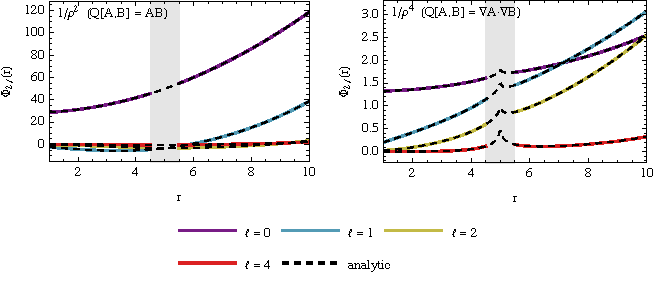
\includegraphics[width=\textwidth]{fig_modes_recovered.pdf}
\caption{Second-order modes $\Phi_{2,\ell}$ (total SS\,+\,SR\,+\,RR) for $\ell=0,1,2,4$.
Solid: recovered by the method. Dashed: analytic.
Left: $Q[A,B]=AB$ ($1/\rho^2$). Right: $Q[A,B]=\nabla A\cdot\nabla B$ ($1/\rho^4$).
Numerical curves are shown in the exterior regions only.
Inside the shaded worldtube the method solves on the contour, where $\tilde\psi(y(a))$ is not the value on the axis.
The cusps near $r_0$ in the right panel are the $\ln|r-r_0|$ singularity of the modes of $q^2/(2\rho^2)$.
In the left panel the $\ell=0$ mode sets the scale, so $\ell=2,4$ lie close to zero.}
\label{fig:modes}
\end{figure}

\begin{figure}[htbp]
\centering
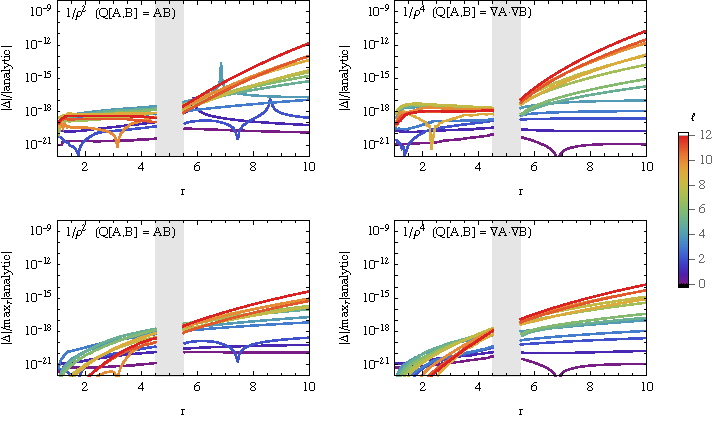
\includegraphics[width=\textwidth]{fig_relative_error.pdf}
\caption{Error of the recovered second-order modes in the exterior regions, for $\ell=0$--$12$ (colour).
Top: pointwise relative error $|\Delta|/|\text{analytic}|$; the isolated spikes are where an analytic mode crosses zero.
Bottom: error scaled by $\max_r|\text{analytic}|$.
The error is at or below $10^{-16}$ for $\ell\le6$.
It grows with $\ell$ and towards $r=10$, reaching $4.0\times10^{-15}$ ($1/\rho^2$) and $1.7\times10^{-14}$ ($1/\rho^4$) at $\ell=12$.}
\label{fig:relerr}
\end{figure}

\begin{figure}[htbp]
\centering
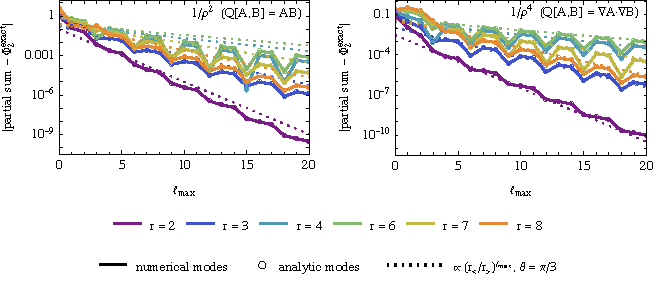
\includegraphics[width=\textwidth]{fig_mode_convergence.pdf}
\caption{Convergence of the 3D mode sum with $\ell_{\max}$, at exterior points $r=2,3,4$ (inside $r_0$) and $r=6,7,8$ (outside), with $\theta=\pi/3$.
Lines: partial sums of the recovered modes. Circles: partial sums of the analytic modes.
The two agree to $1.1\times10^{-15}$ at every point and every $\ell_{\max}$.
So the convergence shown is that of the mode sum itself, not a limitation of the method.
Dotted: $(r_</r_>)^{\ell_{\max}}$, normalised at $\ell_{\max}=4$.
Points nearest the worldtube converge slowest.
The period-3 zig-zag comes from $P_\ell(1/2)$ at $\theta=\pi/3$.}
\label{fig:convergence}
\end{figure}

\clearpage
\section{Truncated punctures defined in 3D}\label{sec:trunc3d}

Section~\ref{sec:shadowtest} used a mode-by-mode truncated puncture.
Here the puncture is a genuine 3D field, used consistently in every piece (condition C3):
\begin{equation}
\Phi^{\rm P}=\frac{q}{\rho}+c\,q\,\rho^n,\qquad n\in\{1,3,5,7\},\qquad c=r_0^{-(n+1)}.
\end{equation}
\begin{itemize}[nosep]
\item Odd powers of $\rho$ are not smooth at $\x_0$, so $cq\rho^n$ mimics a truncation error of order $n$ with expansion scale $r_0$.
\item The residual $\Phi^{\rm res}=\PhiR-cq\rho^n$ now has modes at every $\ell'$.
\item The SS and SR pieces are built from $\Phi^{\rm P}$ in closed form, and RR from $\Phi^{\rm res}$ on the real line.
\end{itemize}
The exterior error splits as before into (a) the real-part mismatch, (b) the shadow contamination, and (c) the truncation of the $\ell'$ coupling sums at $\ell'_{\max}$.

\subsection{Consistent puncture: (a) vanishes, but (b) grows with \texorpdfstring{$\ell'$}{l'}}
\begin{center}
\small
\renewcommand{\arraystretch}{1.15}
\begin{tabular}{@{}llccc@{}}
\toprule
case & $n$ & (b) shadow & (c) $\ell'$ truncation & total\\
\midrule
$1/\rho^2$ & 3 & $4.6\times10^{-5}$ & $2.1\times10^{-3}$ & $2.2\times10^{-3}$\\
$1/\rho^2$ & 7 & $1.5\times10^{-9}$ & $6.2\times10^{-5}$ & $6.2\times10^{-5}$\\
$1/\rho^4$ & 3 & $4.9\times10^{-3}$ & $7.3\times10^{-2}$ & $7.8\times10^{-2}$\\
$1/\rho^4$ & 7 & $2.5\times10^{-7}$ & $1.5\times10^{-3}$ & $1.5\times10^{-3}$\\
\bottomrule
\end{tabular}
\end{center}
These are scaled exterior errors, maximised over $\ell\le6$, with $R=\tfrac12$ and $\ell'_{\max}=12$.
\begin{itemize}[nosep]
\item \emph{(a) is zero in every case}, so the split is exactly consistent.
\item \emph{(b) is linear in $c$}: replacing $c$ by $10c$ multiplies it by $10.00$. At fixed $\ell'_{\max}$ it falls by a factor of about $0.07$--$0.08$ per unit of $n$.
\item \emph{(c) dominates at $\ell'_{\max}=12$.} It converges as a power law, as it would in a real-axis scheme.
\item \emph{(b) does not converge in $\ell'$.} Each mode's contribution grows with $\ell'$.
  Near $\ell'=30$ the growth per mode is $1.13$ ($1/\rho^2$) and $1.19$ ($1/\rho^4$) for $R=\tfrac12$, and $1.06$ and $1.09$ for $R=\tfrac14$.
  These are close to $1+R/r_0$ times a slowly varying power of $\ell'$.
\end{itemize}
\emph{Interpretation} (consistent with the measured rates, but not separately tested).
Under the $\Theta\to H$ continuation, each mode's shadow is built from its inside and outside analytic pieces, which go like $r^{\ell'}$ and $r^{-\ell'-1}$.
Continued across the worldtube, these grow like $(1+R/r_0)^{\ell'}$.
This is the radial analogue of the growth of Legendre polynomials off $[-1,1]$ noted in \nb{Andrew_s_idea.pdf}.

\subsection{Optimum \texorpdfstring{$\ell'_{\max}$}{l'max} and a shrinking worldtube}
Because (c) falls and (b) grows, at fixed $R$ the total error behaves like an asymptotic series.
It reaches a minimum in $\ell'_{\max}$ and then grows, so the best one can do is stop near the optimum.

If instead the worldtube shrinks as modes are added, $R=r_0/\ell'_{\max}$, the amplification $(1+R/r_0)^{\ell'_{\max}}$ stays bounded while the prefactor of (b) goes to zero.
The total then falls monotonically and tracks (c) to within a few per cent (Figure~\ref{fig:lprime}).
\begin{center}
\small
\renewcommand{\arraystretch}{1.15}
\begin{tabular}{@{}llcccc@{}}
\toprule
case & $n$ & $R=\tfrac12$: minimum (at $\ell'_{\max}$) & $R=\tfrac12$ at 40 & $R=\tfrac14$ at 40 & $R=r_0/\ell'_{\max}$ at 40\\
\midrule
$1/\rho^2$ & 3 & $5.7\times10^{-4}$ (20) & $3.5\times10^{-3}$ & $3.1\times10^{-5}$ & $1.0\times10^{-5}$\\
$1/\rho^2$ & 5 & $4.2\times10^{-6}$ (30) & $1.7\times10^{-5}$ & $8.3\times10^{-8}$ & $1.1\times10^{-7}$\\
$1/\rho^4$ & 3 & $0.13$ (20) & $2.8$ & $3.1\times10^{-2}$ & $8.0\times10^{-3}$\\
$1/\rho^4$ & 5 & $1.4\times10^{-3}$ (20) & $1.6\times10^{-2}$ & $2.5\times10^{-5}$ & $6.5\times10^{-5}$\\
\bottomrule
\end{tabular}
\end{center}
These totals were computed from the Lemma~\ref{lem:linear} decomposition by quadrature.
That was checked against full contour solves at two values of $(R,\ell'_{\max})$ per case, to $10^{-14}$.

\begin{figure}[htbp]
\centering
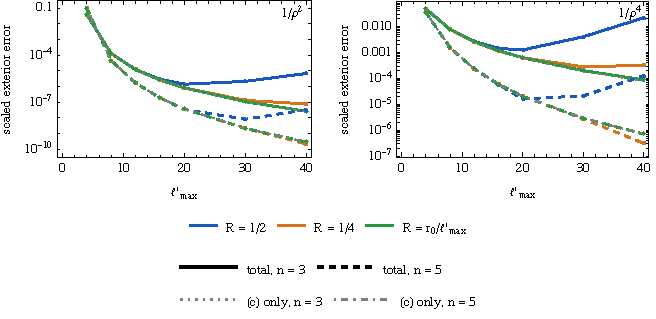
\includegraphics[width=\textwidth]{fig_lprime_optimum.pdf}
\caption{Total exterior error against $\ell'_{\max}$, with the puncture $q/\rho+cq\rho^n$.
Solid: $n=3$. Dashed: $n=5$.
Colours: fixed worldtube $R=\tfrac12$ or $\tfrac14$, and a shrinking worldtube $R=r_0/\ell'_{\max}$.
Dotted: the $\ell'$-truncation error (c) alone.
For fixed $R$ the error has a minimum and then grows, because of the shadow term (b).
With the shrinking worldtube it tracks (c).}
\label{fig:lprime}
\end{figure}

\subsection{The hybrid split}\label{sec:hybrid}
The cross-term (b) arises only because SR is formed on the contour as a product of two shadowed factors.
The hybrid split avoids that product.
Let $T_k\Phi^{\rm res}$ be the 3D Cartesian Taylor polynomial of the residual about $\x_0$, of order $k$. Then
\begin{equation}
2Q[\Phi^{\rm P},\Phi^{\rm res}]
=\underbrace{2Q[\Phi^{\rm P},T_k\Phi^{\rm res}]}_{\text{Part 1}}
+\underbrace{2Q[\Phi^{\rm P},\Phi^{\rm res}-T_k\Phi^{\rm res}]}_{\text{Part 2}}.
\end{equation}
\begin{itemize}[nosep]
\item \emph{Part 1} is closed-form in 3D. It carries every non-integrable or distributional term, and is continued analytically like SS.
  Its coefficients are the residual's local data at $\x_0$, obtained from mode sums at $r_0$.
\item \emph{Part 2} is formed on the real line, where both factors are real.
  It is continued with the extended delta,
  \begin{equation}
  \tilde s(z)=\int_I s(t)\,\dext(z-t)\,dt=\frac{1}{\pi i}\int_I\frac{s(t)}{t-z}\,dt,\qquad I\supset[a_L,a_R].
  \end{equation}
  This is analytic above the axis, and $\Re\tilde s(r+i0)=s(r)$ on $I$ (Plemelj), so Lemma~\ref{lem:linear} applies.
  The interval $I$ extends beyond the worldtube, so the endpoint singularities of the integral lie off the contour.
\end{itemize}
No product of two shadowed factors is ever formed, so (b) is absent (Figure~\ref{fig:hybridschem}).

\paragraph{Why Part 2 is integrable even when SR is not.}
Write $R_k:=\Phi^{\rm res}-T_k\Phi^{\rm res}$.
Here $T_k\Phi^{\rm res}=\Phi^{\rm res}(\x_0)+\Delta x^i\,\partial_i\Phi^{\rm res}(\x_0)+\dots$, to order $k$.
The residual itself is generally non-zero on the worldline, but its value there is the constant term of $T_k$, so it is subtracted.
If $\Phi^{\rm res}$ is $C^{k+1}$ at $\x_0$, Taylor's theorem gives $R_k=O(\rho^{k+1})$, with $\partial^jR_k=O(\rho^{k+1-j})$.
So the remainder, unlike $\Phi^{\rm res}$, vanishes on the worldline to order $k$.
For the puncture $q/\rho+cq\rho^n$ the residual is only $C^{n-1}$, and the statement becomes $R_k=O(\rho^{\min(k+1,n)})$.

Suppose $Q$ puts up to $d$ derivatives on its first argument.
Then each term of $2Q[\Phi^{\rm P},R_k]$ is (derivatives of $\Phi^{\rm P}\sim1/\rho$) $\times$ (derivatives of $R_k$), and every such term is $O(\rho^{k-d})$.
This is locally integrable in 3D when $k-d>-3$, and its distributional derivatives then carry no point-supported part.
Its modes are therefore ordinary integrable functions on the real line, at worst with jumps, and contain no $\delta(r-r_0)$.

Everything non-integrable sits in Part 1, $2Q[\Phi^{\rm P},T_k\Phi^{\rm res}]$.
Part 1 is closed-form and is continued analytically, so its $\delta$ terms appear on the contour as $\dext$ poles and need no special treatment.

For $Q[A,B]=\tfrac12\partial_z^2(AB)$, $d=2$, so $k\ge0$ suffices: subtracting the value $\Phi^{\rm res}(\x_0)$ removes the $\delta$ that comes from $\Phi^{\rm res}(\x_0)\,\partial_z^2(1/\rho)$.
The numerical test of this operator confirms it.

$T_k$ should be built from the same truncated mode sum as the residual that enters Part 2.
The two parts then add back exactly to the truncated SR, so errors in the estimated local data only become part of the ordinary $\ell'$-truncation error.

\begin{figure}[htbp]
\centering
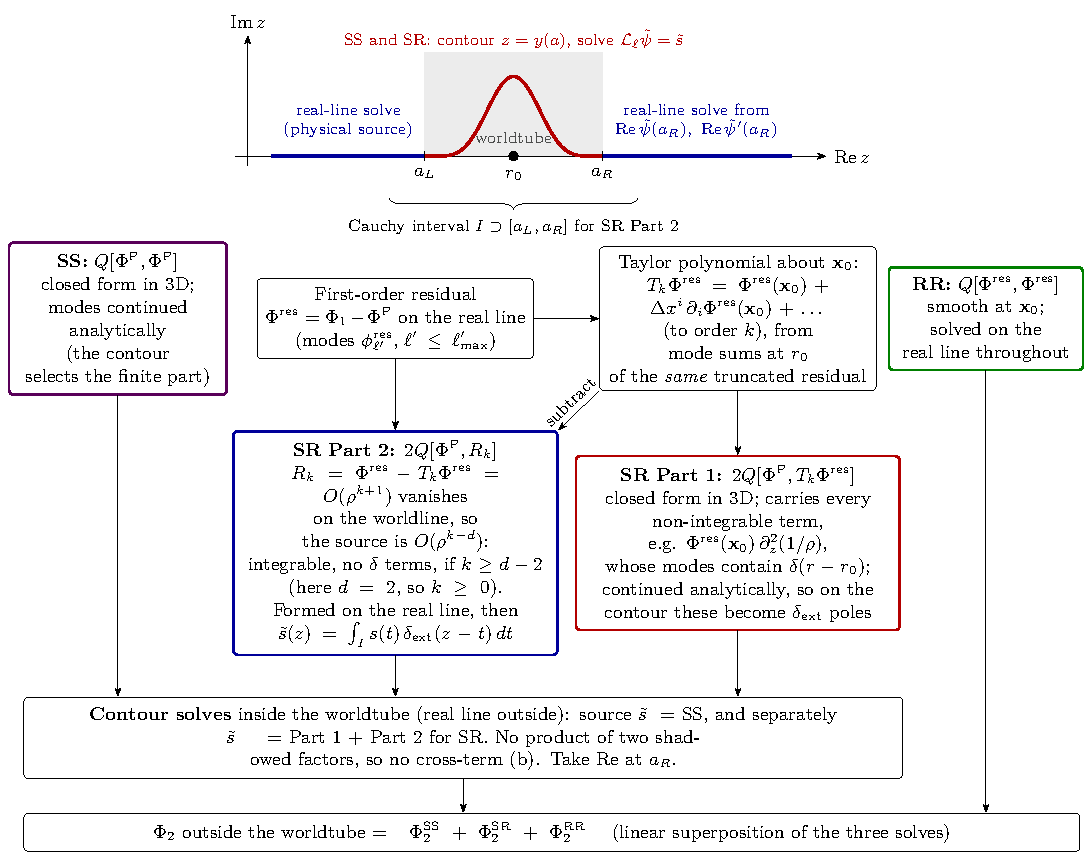
\includegraphics[width=0.92\textwidth]{fig_hybrid_schematic.pdf}
\caption{The second-order pipeline, with the hybrid treatment of SR.
\emph{Top:} the complex $r$-plane. SS and SR are solved on the real line outside the worldtube and on the contour inside it, and the exterior solve restarts from the real part at $a_R$.
\emph{Bottom:} the three pieces.
SS is closed-form and continued analytically.
RR is smooth and solved on the real line throughout.
SR is split in two.
Part~1 carries every non-integrable or distributional term, such as the $\delta(r-r_0)$ in the modes of $\Phi^{\rm res}(\x_0)\,\partial_z^2(1/\rho)$, and is continued analytically.
Part~2 contains $R_k=\Phi^{\rm res}-T_k\Phi^{\rm res}=O(\rho^{k+1})$, which vanishes on the worldline. That makes it integrable, so it can be formed on the real line and Cauchy-continued over an interval $I$ slightly larger than the worldtube.
The exterior second-order field is the sum of the three linear solves.}
\label{fig:hybridschem}
\end{figure}

\paragraph{Results} (puncture order $n=3$, $R=\tfrac12$, scaled error, maximised over $\ell\le6$).
\begin{center}
\small
\renewcommand{\arraystretch}{1.15}
\begin{tabular}{@{}lcc@{}}
\toprule
& $\ell'_{\max}=20$ & $\ell'_{\max}=40$\\
\midrule
$1/\rho^2$, product on the contour & $5.7\times10^{-4}$ & $3.5\times10^{-3}$ (growing)\\
$1/\rho^2$, hybrid & $3.0\times10^{-4}$ & $1.0\times10^{-5}$\\
$1/\rho^4$, product on the contour & $0.13$ & $2.8$ (growing)\\
$1/\rho^4$, hybrid & $5.5\times10^{-2}$ & $7.3\times10^{-3}$\\
\bottomrule
\end{tabular}
\end{center}
\begin{itemize}[nosep]
\item \emph{(b) is gone.}
  In every variant the exterior total equals the $\ell'$-truncation error (c) to better than $10^{-6}$ relative, and it falls monotonically with $\ell'_{\max}$.
  The variants are H0, which Cauchy-continues the whole SR source without a split, and H1 with $k=0,1,2$.
\item \emph{The Cauchy step is accurate.}
  It contributes at most $10^{-14}$, flat in $\ell'_{\max}$, and doubling the resolution changes it by less than $10^{-17}$.
  Getting there required subtracting the cubic Taylor polynomial of $s$ about $\Re z$ (integrated analytically) before Gauss quadrature, and representing the contour source piecewise at 40-digit precision.
  Subtracting only $s(\Re z)$ left a near-singular term and stalled at $10^{-7}$.
\item \emph{The local data converge slowly.}
  Taylor coefficients from mode sums converge only algebraically: at $\ell'_{\max}=40$, $\Phi^{\rm res}(\x_0)$ is off by about $10^{-5}$ and the second derivatives by about $10^{-3}$.
  Here this does not matter, because the estimated polynomial cancels exactly between Parts~1 and~2.
  Section~\ref{sec:dzz} shows the same holds even when SR is distributional, provided $T_k$ is built from the same truncated residual. Inaccurate local data would leave a non-integrable piece in Part~2 only if $T_k$ came from independent data.
\item \emph{Caveat.}
  With $Q=AB$ or $\nabla A\cdot\nabla B$, SR is integrable, so H0 works as well as H1.
  Section~\ref{sec:dzz} tests a distributional SR, where H0 fails and H1 still works.
\end{itemize}

\begin{figure}[htbp]
\centering
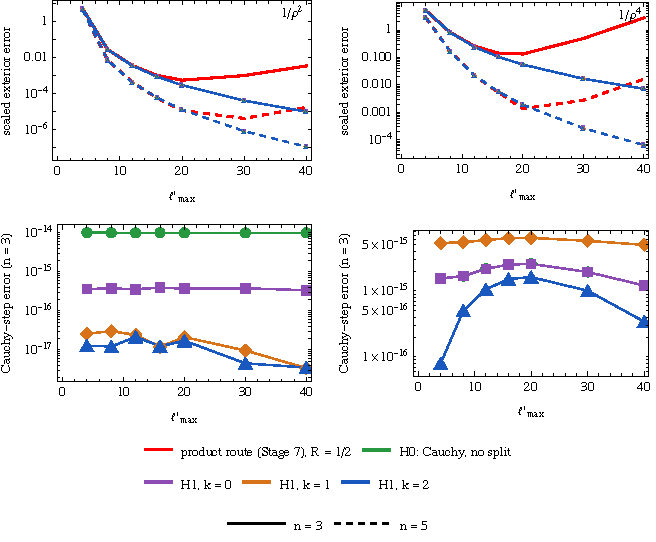
\includegraphics[width=\textwidth]{fig_hybrid.pdf}
\caption{Top: exterior error against $\ell'_{\max}$ for the product route at $R=\tfrac12$ (red) and the hybrid variants. Solid: $n=3$. Dashed: $n=5$.
The hybrid curves converge monotonically and coincide with the $\ell'$-truncation error.
Bottom: error introduced by the Cauchy step ($n=3$), below $10^{-14}$ throughout.}
\label{fig:hybrid}
\end{figure}

\subsection{A distributional SR: \texorpdfstring{$Q[A,B]=\tfrac12\partial_z^2(AB)$}{Q = (1/2) d\_z\^2(AB)}}\label{sec:dzz}

With $Q[A,B]=\tfrac12\partial_z^2(AB)$, the second-order equation is $\nabla^2\Phi_2=\tfrac12\partial_z^2(\Phi_1^2)$.
\begin{itemize}[nosep]
\item \emph{The SR source is realistic.}
  It contains $q\,\Phi^{\rm res}\,\partial_z^2(1/\rho)\sim1/\rho^3$, the same structure as $h^{\rm R}\partial\partial h^{\rm S}$ in self-force.
  This is not integrable as a function, but it is well defined as a distribution, being a second derivative of the locally integrable $\Phi^{\rm res}/\rho$.
\item \emph{Its modes contain $\delta$ terms.}
  The $1/\rho^3$ part averages to zero over angles, so the modes contain $\delta(r-r_0)$ terms rather than a $1/|r-r_0|$ function.
  The modes of $\partial_z$ follow from the ladder $\partial_z(fY_\ell)=a_{\ell+1}(f'-\ell f/r)Y_{\ell+1}+a_\ell(f'+(\ell+1)f/r)Y_{\ell-1}$, with $a_\ell=\ell/\sqrt{(2\ell-1)(2\ell+1)}$.
\item \emph{The exact answer is known.}
  $\partial_z$ commutes with $\nabla^2$, so $\Phi_2=\tfrac12\partial_z^2\chi$, where $\chi$ is the $1/\rho^2$ solution of Section~\ref{sec:numerics}. This holds for any split.
\end{itemize}

\paragraph{Exact puncture ($\ell\le6$).}
SS and SR are recovered on the contour to $5\times10^{-16}$ (scaled), with no point-supported terms: the fitted coefficients are below $2\times10^{-18}$.
The $\delta$ coefficients of the source modes run from $-0.21$ ($\ell=0$) to $-0.77$ ($\ell=6$).
Dropping them, as pointwise sampling of a real-line source does, gives errors of $0.4$ to $500$.

\paragraph{Truncated 3D puncture} ($R=\tfrac12$; scaled exterior error, maximised over $\ell\le6$):
\begin{center}
\small
\renewcommand{\arraystretch}{1.15}
\begin{tabular}{@{}llccc@{}}
\toprule
$n$ & route & $\ell'_{\max}=12$ & $20$ & $40$\\
\midrule
3 & (c) $\ell'$ truncation & $2.2\times10^{-2}$ & $1.6\times10^{-3}$ & $5.0\times10^{-5}$\\
3 & product on the contour & $3.4\times10^{-2}$ & $6.0\times10^{-2}$ (growing) & --\\
3 & H0, no split & $5\times10^{2}$ & $5\times10^{2}$ & $5\times10^{2}$\\
3 & H1, $k=0$--$3$ & $=$ (c) & $=$ (c) & $=$ (c)\\
5 & (c) $\ell'$ truncation & $2.6\times10^{-3}$ & $6.8\times10^{-5}$ & $5.6\times10^{-7}$\\
5 & product on the contour & $2.4\times10^{-3}$ & $5.2\times10^{-4}$ (growing) & --\\
5 & H1, $k=0$--$3$ & $=$ (c) & $=$ (c) & $=$ (c)\\
\bottomrule
\end{tabular}
\end{center}
\begin{itemize}[nosep]
\item \emph{H0 fails}, because the real-line source loses the $\delta$ terms.
  A contour solve confirms the predicted miss exactly ($0.218$ at $\ell=2$, $\ell'_{\max}=8$).
\item \emph{H1 succeeds for every $k$, including $k=0$.}
  Part~2 carries no $\delta$ term (below $10^{-38}$). With $k=0$ it has only a jump at $r_0$; with $k=1$ it is continuous; with $k\ge2$ it is $C^1$.
  This matches the condition $k\ge d-2$ with $d=2$.
\item \emph{Inexact local data do no harm.}
  H1 equals (c) at every $\ell'_{\max}$, although the estimated Taylor value at $\x_0$ is off by $8.5\times10^{-4}$ at $\ell'_{\max}=8$.
  Because $T_k$ is built from the same truncated residual, the $\delta$ cancels exactly between Parts 1 and 2.
\item \emph{The product route degrades sooner} than for $Q=AB$ or $\nabla A\cdot\nabla B$, with its minimum near $\ell'_{\max}=12$--$16$.
  The second $z$-derivative amplifies the shadow of the high-$\ell'$ modes.
\end{itemize}

\begin{figure}[htbp]
\centering
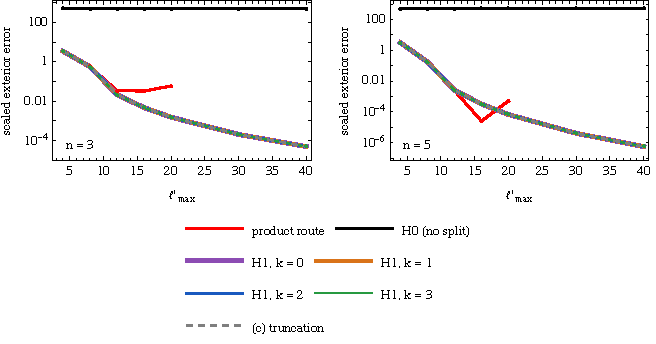
\includegraphics[width=\textwidth]{fig_dzz.pdf}
\caption{Distributional SR, $Q[A,B]=\tfrac12\partial_z^2(AB)$.
Exterior error against $\ell'_{\max}$ for $n=3$ (left) and $n=5$ (right), with $R=\tfrac12$.
H0, the real-line source with no split, fails at the $5\times10^2$ level because it misses the $\delta(r-r_0)$ terms.
The hybrid split H1 ($k=0$--$3$) coincides with the $\ell'$-truncation error (c) (dashed).
The product route on the contour follows (c) until the shadow term takes over, near $\ell'_{\max}=12$--$16$.}
\label{fig:dzz}
\end{figure}

\paragraph{The two remedies compared.}
\begin{itemize}[nosep]
\item The shrinking worldtube needs no extra data, and it suppresses (b).
\item The hybrid split removes (b) entirely. When SR is distributional, it needs the residual's local data at the particle, built from the same truncated mode sum. Their accuracy then enters only through the ordinary $\ell'$ truncation.
\end{itemize}

\clearpage
\section{Relation to recent work: Musaeus, Pound and Upton (2026); Upton et al.\ (2026)}\label{sec:mpu}

Ref.~\cite{MusaeusPoundUpton2026} gives a rigorous point-particle (``skeletonised'') form of the second-order Einstein equation.
It shows that the second-order source can be handled with off-the-shelf regularisation, without a puncture.
Several of its results bear directly on this note.

\subsection{What the paper establishes}
\begin{itemize}[nosep]
\item \emph{The same split.}
  The quadratic source is split into SS, SR and RR pieces (their eq.~18), exactly as in~\eqref{eq:split}.
  SR, $2Q_{\rm R}[h^{\rm S(1)}]$, is a linear operator acting on the integrable $h^{\rm S(1)}$, so it is well defined as a distribution.
  SS is defined as $-\delta G[h^{\rm SS}]$, again a linear operator on an integrable function.
\item \emph{The structure of SR.}
  The leading SR term is $k^{\alpha\beta}{}_{\mu\nu}\hat n^{\mu\nu}/\rho^3$ (their eq.~35). Its angular part $\hat n^{\mu\nu}$ is symmetric and trace-free, so it integrates to zero over the sphere, and the $1/\rho^2$ terms have odd parity.
  At mode level, SR terms consist of jumps, $\delta$ functions and their derivatives (their Sec.~V.C).
  This answers the question left open in the previous version of this note: the flat-toy picture of Section~\ref{sec:dzz} carries over to self-force, with no non-integrable $1/|r-r_0|$ functions.
\item \emph{The prescription.}
  The canonical distributional source equals the Hadamard \emph{partie finie} plus a finite worldline term (their eq.~24):
  \begin{equation}
  \hat\delta^2G^{\alpha\beta}=\mathrm{Pf}\,\delta^2G^{\alpha\beta}+8\pi T^{\alpha\beta}_Q,
  \end{equation}
  where $T_Q$ is built from $h^{\rm R(1)}$ on the worldline.
  At mode level the finite part reduces to subtracting the $A_{\ell m}/\Delta r^2$ and $B_{\ell m}/\Delta r$ terms and integrating by parts (their eqs.~105--112).
  For Teukolsky sources the singular terms go up to $1/\Delta r^4$.
\end{itemize}

\subsection{Benchmark 1: the contour reproduces their mode-level finite part}
Their Sec.~V.D treats a static particle in flat space with the spin-weight $-2$ radial Teukolsky operator $r^2\partial_r^2-2r\partial_r-(\ell-1)(\ell+2)$ and the Green's function of their eq.~140.
We used sources $A/\Delta r^4+B/\Delta r^3+C/\Delta r^2+D/\Delta r$ (each term singly, and mixed) for $\ell=2$--$6$, and computed the solution outside the worldtube in three ways:
\begin{enumerate}[nosep,label=P\arabic*.]
\item their finite-part prescription, eqs.~141 and A2--A5;
\item their closed form for $\ell=2$, eq.~142;
\item the contour: $\Re\int_C G(r,z)S(z)\,dz$ plus the real-line integral outside the worldtube.
\end{enumerate}
\begin{itemize}[nosep]
\item P1 agrees with an independent, Taylor-subtracted finite part to below $10^{-38}$, and is independent of the cutoff $a$.
\item Eq.~142 is correct as printed.
\item The contour agrees with P1 to $4\times10^{-34}$ or better for every source, every $\ell$ and five choices of worldtube radius and contour amplitude. A contour ODE solve agrees to $8\times10^{-16}$.
\end{itemize}
This is expected: the boundary value of $(\Delta r+i0)^{-n}$ has the Hadamard finite part as its real part.
So the contour is an automatic implementation of their mode-level regularisation, including the $1/\Delta r^3$ and $1/\Delta r^4$ singularities of Teukolsky-type sources, with no coefficients to compute and no integrations by parts.
It also generalises the Stage~5 finding of Section~\ref{sec:numerics4}, which is the toy counterpart of their eq.~86.

\subsection{Benchmark 2: \texorpdfstring{$T_Q$}{T\_Q} in the \texorpdfstring{$\partial_z^2$}{d\_z\^2} toy}
For $Q[A,B]=\tfrac12\partial_z^2(AB)$ with the exact puncture, the SR piece is $q\,\partial_z^2(\PhiR/\rho)$.
\begin{itemize}[nosep]
\item \emph{The toy $T_Q$.}
  Using $\partial_z^2(1/\rho)=\mathrm{PV}\,(3n_z^2-1)/\rho^3-\tfrac{4\pi}{3}\delta^3$, the canonical SR minus the 4D finite part of the pointwise SR is
  \begin{equation}
  T_Q^{\rm toy}=-\tfrac{4\pi}{3}\,q\,\PhiR(\x_0)\,\delta^3(\x-\x_0),
  \end{equation}
  verified to $10^{-21}$. It is the analogue of their $T_Q$: a worldline term linear in the regular field at the particle.
\item \emph{How the mode-level $\delta$ splits.}
  The $\delta(r-r_0)$ coefficient found in the SR source modes in Stage~9 is $c_\ell=-4\pi q\PhiR(\x_0)Y_\ell(0)/r_0^2$.
  It splits exactly into $\tfrac23c_\ell$ from the 4D finite part and $\tfrac13c_\ell$ from $T_Q$, both to $10^{-20}$.
  The $\tfrac23$ arises because the 4D finite part excludes a ball around the particle, whereas mode functions effectively integrate over spherical shells, which near the particle act like slabs.
\end{itemize}

Scaled exterior errors for $\ell\le6$ are below; ``modes'' means the source modes used.
\begin{center}
\small
\renewcommand{\arraystretch}{1.15}
\begin{tabular}{@{}lc@{}}
\toprule
prescription & error\\
\midrule
contour (canonical source, no $T_Q$ needed) & $<10^{-27}$\\
modes of the 4D finite part $+\;T_Q$ (their eq.~24) & $<10^{-17}$\\
modes of the 4D finite part, no $T_Q$ & $0.14$ to $170$\\
pointwise modes with the mode-level finite part (their eq.~105) $+\;T_Q$ & $0.27$ to $340$\\
pointwise modes, no $\delta$ terms at all & $0.41$ to $500$\\
\bottomrule
\end{tabular}
\end{center}

\paragraph{A subtlety in the mode-level reduction.}
Their eq.~24 is exact in the toy, but only if the mode functions are those of the 4D finite-part \emph{distribution}, including its $\delta$ content.
In the step from eq.~104 to eq.~105, the ball regulator $(\rho/\rho_0)^B$ is dropped once $|\Delta\tilde r|^{B'}$ is inserted.
For the trace-free $1/\rho^3$ term the two regulators do not commute: a term proportional to $B'/(B+B')$ survives.
Applied to pointwise mode functions, eq.~105 therefore gives a ``slab'' result equal to the 4D finite part plus $\tfrac{8\pi}{3}q\PhiR(\x_0)\delta^3$. Adding $T_Q$ then misses $\tfrac23c_\ell$.

There are three ways of book-keeping the source modes, and only two are consistent:
\begin{itemize}[nosep]
\item modes of the 4D finite part, plus $T_Q$;
\item modes of the canonical distribution, for example built by applying the differential operator to kinked mode functions, \emph{without} adding $T_Q$, which would double-count it;
\item pointwise modes, which need $T_Q$ \emph{and} the finite part's own $\delta$ content added back. These are inconsistent if only $T_Q$ is added.
\end{itemize}
The paper's Sec.~V.D example has $h^{\rm R}=0$, so $T_Q=0$, and the subtlety does not arise there, consistent with Benchmark~1.
Whether it matters in practice in GR depends on how $\delta^2G_{\ell m}$ is constructed.
This is a toy-model observation that may be worth raising with the authors.

\subsection{What this means for the contour method}
\begin{itemize}[nosep]
\item The contour reproduces the paper's mode-level regularisation exactly, including Teukolsky-type $1/\Delta r^4$ sources.
\item If the SS and SR source modes are built as operators acting on continued integrable mode functions, as in our product route and in Part~1 of the hybrid split, the contour yields the canonical source directly. The worldline terms then appear as $\dext$ poles, with no separate $T_Q$ and no risk of double counting.
\item For the metric-level source, Part~1 of the hybrid split needs only $h^{\rm R(1)}$ on the worldline ($k=0$). That is the same datum that enters $T_Q$ and the first-order self-force.
  Teukolsky sources carry up to two more derivatives, giving $\delta'$ and $\delta''$ terms. These need $k=2$, or the source operator moved onto the Green's function by parts, as the paper suggests.
\item The paper's real-axis route needs no contour, only the local singular coefficients and $T_Q$.
  The contour's advantages are automatic regularisation of any order of pole, automatic handling of $\delta$ terms, and natural use of the SS/SR/RR split against slow mode coupling.
  Its costs are that it needs continuable source modes, and that truncated punctures produce the shadow effects of Section~\ref{sec:trunc3d}.
\item The paper notes that at third order $h^{(n)}\sim1/\rho^n$ is no longer locally integrable, so its linear-operator construction fails.
  Analytic continuation does not rely on local integrability, so the contour might extend further. That is speculative and untested.
\end{itemize}

\subsection{The production effective source of Upton et al.\ (2026)}\label{sec:upton}
Ref.~\cite{Upton2026} describes the second-order effective source behind the first post-adiabatic waveform calculations: Lorenz gauge, quasicircular orbits in Schwarzschild, and a real-axis puncture scheme.
Three points bear on this note.

\paragraph{1. It confirms the consistency conditions.}
Inside a worldtube, the second-order Ricci tensor is split into RR, SR, RS and SS pieces using $h^1=h^{\rm P1}+h^{\rm R1}$ (their eq.~177), as in~\eqref{eq:splitP}.
They stress two requirements:
\begin{itemize}[nosep]
\item the \emph{same} puncture and residual must be used in all four terms;
\item the puncture's mode decomposition must be exact, ``not a series expansion in $\Delta r$''.
\end{itemize}
These are condition (C3) and the lesson of the mode-by-mode Taylor puncture in Section~\ref{sec:shadowtest}.
Their puncture is multiplied by an angular window function, which is the freedom allowed in Section~\ref{sec:traditional}.
Their SR and RS mode-coupling sums converge polynomially in $\ell_{\max}$, by the same mechanism as our $\ell'$-truncation error (c).
Their balance between worldtube size and $\ell_{\max}$ mirrors Section~\ref{sec:trunc3d}, without the shadow term, since everything is on the real axis.

\paragraph{2. It shows how the source modes are built in practice.}
They interpret radial derivatives of the mode functions distributionally, with $\partial_r^2|\Delta r|=2\delta(\Delta r)$.
They extract the $\delta$ content of the mode-coupled SR sums, and check that it matches the stress-energy $\delta$ terms (their Fig.~13).
This is the ``canonical'' book-keeping of Section~\ref{sec:mpu}, so the mode-level subtlety found there does not affect their puncture-scheme results.
It does matter for anyone combining such mode-coupled sources with eq.~24 of Ref.~\cite{MusaeusPoundUpton2026}: those modes already contain the $T_Q$ $\delta$, so adding $8\pi T_Q$ again would double-count it.
Their $\bar T^{\rm QRic}$ (eq.~A28) arises from the same kind of $K^Q$ boundary term as $T_Q$, and appears to be the GR counterpart of the toy $T_Q$; in their formulation it sits in the field equation for $h^{\rm SR}$ (eq.~54).

\paragraph{3. Where the contour could help in GR, and where it could not.}
Their dominant cost is the SS piece: two-dimensional numerical angular integrals of $\delta^2R[h^{\rm P1},h^{\rm P1}]$ on a real-$r$ grid, about $3\times10^6$ CPU hours.
Much of the remaining effort goes into the second-order puncture $h^{\rm P2}$ and its many pieces and jump checks.
\begin{itemize}[nosep]
\item \emph{What the contour would remove.}
  It needs no $h^{\rm P2}$: continuation regularises SS and SR directly. It also handles $\delta$ terms automatically.
\item \emph{What it would not remove.}
  The contour needs every source as a function it can evaluate at complex $z=y(a)$.
  In the toy the SS modes are closed-form (Legendre $Q_\ell$ functions), so they are continued directly.
  In GR they exist only as numbers on a real grid, which cannot be evaluated off the axis.
  So the SS mode integrals are still needed, and in addition must be put into a form that can be continued.
\end{itemize}

\paragraph{Reusing the hybrid technique for SS.}
The mechanism of the hybrid split can solve this availability problem: a closed-form singular part continued analytically, plus an integrable remainder known on the real line and continued by the Cauchy integral $\int s(t)\,\dext(z-t)\,dt$.
Mode by mode:
\begin{itemize}[nosep]
\item \emph{Singular part:} $A_{\ell m}/\Delta r^2+B_{\ell m}/\Delta r$, with coefficients from the local 4D expansion. These are the same coefficients as in eq.~109 of Ref.~\cite{MusaeusPoundUpton2026}. This part is continued exactly, and the contour takes its finite part.
\item \emph{Remainder:} the numerical SS modes minus the singular part. It is at worst $\ln|\Delta r|$, so it is integrable and can be Cauchy-continued.
\end{itemize}
The \emph{motivation} differs from the SR case:
\begin{center}
\small
\renewcommand{\arraystretch}{1.2}
\begin{tabular}{@{}>{\raggedright}p{2.4cm}>{\raggedright}p{6.0cm}>{\raggedright\arraybackslash}p{6.0cm}@{}}
\toprule
& SR (tested, Sections~\ref{sec:hybrid}--\ref{sec:dzz}) & SS (GR proposal)\\
\midrule
problem & a product of two continued factors produces the shadow cross-term (b) & the source is known only numerically on the real line, so it cannot be evaluated on the contour\\
Part 1 (closed form) & $2Q[\Phi^{\rm P},T_k\Phi^{\rm res}]$, from local Taylor data of the residual & $A_{\ell m}/\Delta r^2+B_{\ell m}/\Delta r$, from local singular coefficients\\
Part 2 (Cauchy-continued) & $2Q[\Phi^{\rm P},\Phi^{\rm res}-T_k\Phi^{\rm res}]$ & SS minus its singular part\\
\bottomrule
\end{tabular}
\end{center}
SS has no shadow cross-term: it is built from the 3D/4D puncture expression, not from a product of continued fields.
Only the mechanism is shared.

Subtracting $A_{\ell m}/\Delta r^2+B_{\ell m}/\Delta r$ and handling it analytically is essentially the Hadamard procedure of Ref.~\cite{MusaeusPoundUpton2026}.
So for SS in GR the contour adds little beyond that route, and the expensive SS mode integrals remain either way.
Its gains in GR would be the absence of $h^{\rm P2}$ and the automatic treatment of $\delta$ terms.
The optimisations proposed in Ref.~\cite{Upton2026} would help a contour approach just as much: subtracting at 4D level before decomposing, doing one angular integral analytically, or using an $m$-mode scheme.

\paragraph{Teukolsky sources.}
Ref.~\cite{Upton2026} carries the puncture two orders further specifically for second-order Teukolsky sources, because those carry two extra derivatives.
That matches the requirement $k=2$ for Part 1 of the hybrid split in the Teukolsky case.

\clearpage
\section{Next steps}\label{sec:next}
\begin{enumerate}[nosep]
\item \emph{The real static-particle Teukolsky source.} Repeat Benchmark~1 with the actual $-2T_{\ell m}$ derived from $\delta^2G$, not a model source.
\item \emph{Test the SS reuse of the hybrid technique.} In the toy, build the SS source on the contour as an analytic singular part plus a Cauchy-continued remainder, treating the remainder as if known only numerically on the real line. Then compare with the closed-form continuation (Section~\ref{sec:upton}).
\item \emph{Optionally, use a massive scalar}, $(\nabla^2-\mu^2)\Phi=-4\pi q\delta^3$. Its singular field $qe^{-\mu\rho}/\rho$ truncates naturally, giving a realistic 3D puncture in place of the artificial $cq\rho^n$.
\item \emph{Port the fixes back to the original notebook:}
  \begin{itemize}[nosep]
  \item use $\phiS_\ell=\psi_p-D_\ell$;
  \item rewrite the logarithms onto the correct branch;
  \item use the normalisation $\kappa_\ell$;
  \item keep $\Im\tilde\phi^{\rm R}(a_R)$ as a diagnostic instead of discarding it with \code{Re[valR]}.
  \end{itemize}
\end{enumerate}

\begin{thebibliography}{9}
\bibitem{BarackGolbourn2007}
L.~Barack and D.~A.~Golbourn,
``Scalar-field perturbations from a particle orbiting a black hole using numerical evolution in 2+1 dimensions,''
Phys.\ Rev.\ D \textbf{76}, 044020 (2007).

\bibitem{VegaDetweiler2008}
I.~Vega and S.~Detweiler,
``Regularization of fields for self-force problems in curved spacetime: foundations and a time-domain application,''
Phys.\ Rev.\ D \textbf{77}, 084008 (2008).

\bibitem{MillerWardellPound2016}
J.~Miller, B.~Wardell and A.~Pound,
``Second-order perturbation theory: the problem of infinite mode coupling,''
Phys.\ Rev.\ D \textbf{94}, 104018 (2016).

\bibitem{MusaeusPoundUpton2026}
J.~Musaeus, A.~Pound and S.~D.~Upton,
``Point particles in general relativity: beyond linear perturbation theory,''
arXiv:2609.10521 [gr-qc] (2026).

\bibitem{Upton2026}
S.~D.~Upton, B.~Wardell, A.~Pound, N.~Warburton and L.~Barack,
``Effective source for second-order self-force calculations: quasicircular orbits in Schwarzschild spacetime,''
arXiv:2508.00087v2 [gr-qc] (2026).
\end{thebibliography}

\end{document}
